\documentclass[11pt,a4paper,oldfontcommands,oneside]{memoir}
\RequirePackage[english]{babel}
\usepackage[utf8]{inputenc}
\usepackage[T1]{fontenc}
\usepackage{microtype}
\usepackage{graphicx}
\usepackage{xcolor}
\usepackage{times}

\usepackage{url}
\usepackage{afterpage}
\usepackage{pstool}
\usepackage{comment}
\usepackage{wrapfig}
\usepackage[printonlyused]{acronym}
\usepackage{listings}
\usepackage{placeins}

\usepackage[
breaklinks=true,colorlinks=true,
linkcolor=blue,urlcolor=blue,citecolor=blue,% PDF VIEW
%linkcolor=black,urlcolor=black,citecolor=black,% PRINT
bookmarks=true,bookmarksopenlevel=2]{hyperref}

\usepackage{geometry}
% PDF VIEW
% \geometry{total={210mm,297mm},
% left=25mm,right=25mm,%
% bindingoffset=0mm, top=25mm,bottom=25mm}
% PRINT
\geometry{total={210mm,297mm},
left=20mm,right=20mm,
bindingoffset=10mm, top=25mm,bottom=25mm}


%\OnehalfSpacing
%\linespread{1.3}

%%% CHAPTER'S STYLE
\chapterstyle{bianchi}
%\chapterstyle{ger}
%\chapterstyle{madsen}
%\chapterstyle{ell}
%%% STYLE OF SECTIONS, SUBSECTIONS, AND SUBSUBSECTIONS
\setsecheadstyle{\Large\bfseries\sffamily\raggedright}
\setsubsecheadstyle{\large\bfseries\sffamily\raggedright}
\setsubsubsecheadstyle{\bfseries\sffamily\raggedright}


%%% STYLE OF PAGES NUMBERING
%\pagestyle{companion}\nouppercaseheads
%\pagestyle{headings}
%\pagestyle{Ruled}
\pagestyle{plain}
\makepagestyle{plain}
\makeevenfoot{plain}{\thepage}{}{}
\makeoddfoot{plain}{}{}{\thepage}
\makeevenhead{plain}{}{}{}
\makeoddhead{plain}{}{}{}

\setlength{\parindent}{0em}
\setlength{\parskip}{0.7em}

\maxsecnumdepth{subsection} % chapters, sections, and subsections are numbered
\maxtocdepth{subsection} % chapters, sections, and subsections are in the Table of Contents


\begin{document}
%%%---%%%---%%%---%%%---%%%---%%%---%%%---%%%---%%%---%%%---%%%---%%%---%%%
%   TITLEPAGE
%
%   due to variety of titlepage schemes it is probably better to make titlepage manually
%
%%%---%%%---%%%---%%%---%%%---%%%---%%%---%%%---%%%---%%%---%%%---%%%---%%%
\thispagestyle{empty}

{%%%
\sffamily
\centering
\Large

~\vspace{\fill}
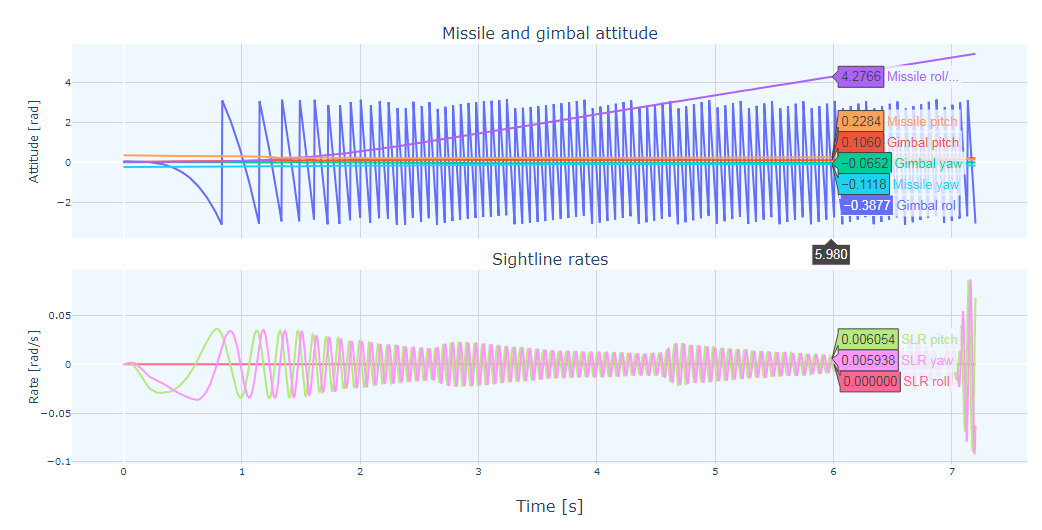
\includegraphics[width=0.90\textwidth]{pic/graphs}

{\huge
Dash Line Plot Python Graphing Utility
}

\vspace{2.5cm}

{\LARGE
MS Willers
}
\vspace{0.5cm}

riana.willers@deneldynamics.co.za\\
riana.willers@gmail.com

\vspace{3.5cm}

Collaborator: CJ Willers
\vspace{0.5cm}

nwillers@csir.co.za\\
neliswillers@gmail.com

\vspace{3.5cm}

\vspace{\fill}

March 2020

%%%
}%%%

\clearpage
%%%---%%%---%%%---%%%---%%%---%%%---%%%---%%%---%%%---%%%---%%%---%%%---%%%
%%%---%%%---%%%---%%%---%%%---%%%---%%%---%%%---%%%---%%%---%%%---%%%---%%%

\tableofcontents*

\clearpage

\listoffigures*


% -*- TeX -*- -*- UK -*- -*- Soft -*-
% use:
%  \ac{IR}

% use template-defined width if defined, else, use AAAA defined below
\ifdef{\acrofirstcolwidth}{}{\newcommand{\acrofirstcolwidth}{AAAA}}
\ifdef{\abbrevitemssep}{}{\newlength{\abbrevitemssep}\setlength{\abbrevitemssep}{0pt}}

\begingroup
% to get wider first column add more AAA to the option
% to adjust vertical spacing adjust itemsep
\begin{acronym}[\acrofirstcolwidth]\itemsep=\abbrevitemssep
\acro{1-D}{One-Dimensional}
\acro{1D}{One-Dimensional}
\acro{2-D}{Two-Dimensional}
\acro{2D}{Two-Dimensional}
\acro{3-D}{Three-Dimensional}
\acro{3D}{Three-Dimensional}
\acro{6-DOF}{Six Degrees of Freedom}
\acro{6DOF}{Six Degrees of Freedom}
\acro{A2D}{Analogue to Digital}
\acro{AA}{Air-to-Air}
\acro{AAM}{Air-to-Air Missile}
\acro{AASRAM}{Air-to-Air Short Range Missile}
\acro{ABF}{Absolute Bloody Final}
\acro{ABL}{Airborne Laser}
\acro{AC}{Alternating Current}
\acro{ACE}{Adaptive Communication Environment}
\acro{AD}{Analogue to Digital (conversion)}
\acro{ADC}{Analogue to Digital Converter}
\acro{AFB}{Air Force Base}
\acro{AFCRL}{Air Force Cambridge Research Laboratories}
\acro{AFRL}{Air Force Research Laboratories}
\acro{AGC}{Automatic Gain Control}
\acro{AGL}{Above Ground Level}
\acro{AGT}{Atmosphere Generator Toolkit}
\acro{AHP}{Analytical Hierarchy Process}
\acro{AI}{Artificial Intelligence}
\acro{AIM}{Air Intercept Missile}
\acro{AIRS}{Atmospheric Infrared Sounder}
\acro{ALG}{Atmospheric Look-up Table Generator}
\acro{AM}{Amplitude Modulation}
\acro{AMBBB}{Ambient Temperature Blackbody}
\acro{AMRAAM}{Advanced Medium Range Air-to-Air Missile}
\acro{ANSI}{American National Standards Institute}
\acro{AOT}{Aerosol Optical Thickness}
\acro{API}{Application Programming Interface}
\acro{APU}{Auxiliary Power Unit}
\acro{ARLBED}{Army Research Laboratory Battlefield Environment Directorate}
\acro{ASCII}{American Standard Code for Information Interchange}
\acro{ASIC}{Application Specific Integrated Circuit}
\acro{ASL}{Above Sea Level}
\acro{ASRAAM}{Advanced Short Range Air-to-Air Missile}
\acro{ASU}{Air Support Unit}
\acro{ATBD}{Algorithm Theoretical Basis Document}
\acro{ATK}{Aerosol toolkit}
\acro{ATP}{Acceptance Test Procedure}
\acro{ATRept}[ATR]{Acceptance Test Report}
\acro{ATR}[ATR]{Automatic Target Recognition}
\acro{ATS}{Advanced Thermographic Systems}
\acro{AU}{Astronomical Unit}
\acro{AVI}{Audio Video Interleave}
\acro{BAe}{British Aerospace}
\acro{BB}{Black Body}
\acro{BCU}{Battery Coolant Unit}
\acro{BDI}{Buffered Direct Injection}
\acro{BFS}{Bomem File System}
\acro{BGRAMS}{Bomem Grams a software product}
\acro{BGT}{Bodenseewerk Ger\"atetechnik Gmbh}
\acro{BH}{I/O Bulkhead input/output}
\acro{BIT}{Built-in Test}
\acro{BLT}{Bilinear Transformation}
\acro{BNC}{Bayonet Neill-Concelman}
\acro{BP}{Blue Test Point}
\acro{BPDF}{Bidirectional Polarization Distribution Functions}
\acro{BPR}{Bad Pixel Replacement}
\acro{BRDF}{Bidirectional Reflectance Distribution Function}
\acro{BSD}{Berkeley Source Distribution}
\acro{BSP}{Binary Space Partitions}
\acro{BVR}{Beyond Visual Range}
\acro{C2}[C$^2$]{Command and Control}
\acro{C3}[C$^3$]{Command,  Control and Communication}
\acro{C3ISTAR}[C$^3$ISTAR]{Command, Control, Communications, Intelligence, Surveillance, Target Acquisition and Reconnaissance}
\acro{C4I3RS}[C$^4$I$^3$RS]{Command, Control, Communication, Computers, Information, Intelligence, Informatics, Reconnaissance and Surveillance}
\acro{CAD}{Computer Aided Design}
\acro{CAE}{Canadian Aviation Electronics}
\acro{CAMEO-SIM}{CAMoflauge Electro-Optic Simulator}
\acro{CAT}{Computed Axial Tomography}
\acro{CCD}{Charge Coupled Device}
\acro{CCIR}{Comite Consultatif International des Radio Communications}
\acro{CCM}{Counter-countermeasure}
\acro{CD}{Compact Disk}
\acro{CDB}{Common Database Standard}
\acro{CDS}{Correlated Double Sampling}
\acro{CDSD}{Carbon Dioxide Spectroscopic Database}
\acro{CEDIP}{Name of the camera manufacturer}
\acro{CFAR}{Constant False Alarm Rate}
\acro{CFD}{Computational Fluid Dynamics}
\acro{CFI}{Customer Furnished Information}
\acro{CHIMES}{Cranfield Hyperspectral Image Modelling and Evaluation System}
\acro{CIGI}{Common Image Generator Interface}
\acro{CML}{Configurable Math Library}
\acro{CMOS}{Complementary Metal Oxide Semiconductor}
\acro{CMS}{Classified MicroSeek}
\acro{CmSim}{Countermeasure Simulator (version 1)}
\acro{CmSim2}{Countermeasure Simulator (version 2)}
\acro{CMT}{Cadmium Mercury Telluride}
\acro{CnC}{Command and Control}
\acro{CNES}{Centre National d'Etudes Spatiales, France}
\acro{CNR}{Clutter-to-noise ratio}
\acro{CNUC}{Continuous Non-Uniformity Correction}
\acro{CO$_2$}{Carbon Dioxide}
\acro{CODATA}{Committee on Data for Science and Technology}
\acro{COM}{Common Object Model}
\acro{COMBIC}{Combined Obscuration Model for Battlefield Contaminants}
\acro{ConOps}{Concept of Operations}
\acro{CORBA}{Common Object Request Broker Architecture}
\acro{COTS}{Commercial of the Shelf}
\acro{CPU}{Central Processing Unit}
\acro{CSCI}{Computer Software Configuration Item}
\acro{CSIR}{Council for Scientific and Industrial Research}
\acro{css}{cascading style sheet}
\acro{CSV}[CSV]{Comma Separated Variable}
\acro{csv}[CSV]{comma-separated-values}
\acro{CTAN}{Comprehensive TeX Archive Network}
\acro{CTIA} {Capacitive Transimpedance Amplifiers}
\acro{CUDA}{Compute Unified Device Architecture}
\acro{CVD}{Chemical vapour deposition}
\acro{CVS}{Concurrent Versions System}
\acro{DARPA}{Defense Advanced Research Projects Agency}
\acro{DAS}{Denel Aerospace }
\acro{DC}{Direct Current}
\acro{DCM}{Direction Cosine Matrix}
\acro{DCS}{Direct Current Subtraction}
\acro{DD}{Denel Dynamics}
\acro{DEM}{Digital Elevation Map}
\acro{DEMS}{Digital Elevation Maps}
\acro{DFPN}{Dark current Fixed Pattern Noise}
\acro{DFT} {Discrete Fourier Transform}
\acro{DGA}{Direction Generale de l'Armement}
\acro{DI}{Direct Injection}
\acro{DIRCM}{Directed Infrared Countermeasure}
\acro{DIRSIG}{Digital Imaging and Remote Sensing Image Generation}
\acro{DIS}{Distributed Interactive Simulation}
\acro{DISORT}{Discrete Ordinates Radiative Transfer Program for a Multi-Layered Plane-Parallel Medium}
\acro{DITSIM}{Directed Infrared Countermeasure and Imaging Toolkit Simulator}
\acro{dl}[DL]{Digital Level}
\acro{DL}[DL]{Digital Level}
\acro{DLE}{Differential Linearity Error }
\acro{DLea}[DL]{Deep Learning}
\acro{DLL}{Dynamic Load Library}
\acro{DLSWC}{Denel Land Systems Western Cape}
\acro{DLU}{Directed Laser Unit}
\acro{DoD}{Department of Defense}
\acro{DOI}{Digital Object Identifier}
\acro{DOTR}{Denel Overberg Test Range}
\acro{DPA}{Digital Processing Assembly}
\acro{DPSS}{Defence, Peace Safety and Security, an operating unit of the CSIR}
\acro{DRI}{Detection, Recognition and Identification}
\acro{DRY}{Don't Repeat Yourself}
\acro{DSIM}{Directed Infrared Countermeasure Simulator}
\acro{DSMC}{Direct Simulation Monte Carlo}
\acro{DSP}{Digital Signal Processing}
\acro{DSTO}{Defense Science and Technology Organisation}
\acro{DTD}{Document Type Definition}
\acro{DTV}{Digital Television}
\acro{DTw}{Digital Twin}
\acro{DVD}{Digital Video Disk or Digital Versatile Disk}
\acro{ECCM}{Electronic Counter-Countermeasure}
\acro{ECEF}{Earth Centred Earth Fixed}
\acro{EDERI}{Electronic Defence Evaluation and Research Institute}
\acro{EDS}{Electronic Defence Systems}
\acro{EEPROM}{Electronically Erasable Programmable Read-Only Memory}
\acro{EGT}{Exhaust Gas Temperature}
\acro{EICAS}{Engine Indication and Crew Alert System}
\acro{EMC}{Electromagnetic Compatibility}
\acro{EME}{Environmental Modelling Editor}
\acro{EMEA}{Europe, Middle East, and Africa}
\acro{EMF}{Electromotive force}
\acro{EMI}{Electro-magnetic interference}
\acro{EMP}{Electro-magnetic pulse}
\acro{ENU}{East North Up}
\acro{ENVI}{An image processing product}
\acro{EO}{Electro Optic(s/al)}
\acro{EofN}{east of north}
\acro{EOSS}{Electro-Optical Simulation System}
\acro{EPS}{European Polar System }
\acro{EPW}{Energy Plus Weather}
\acro{ESA}{European Space Agency}
\acro{ESD}{East-South-Down (coordinate convention)}
\acro{ESRL}{Earth System Research Laboratory}
\acro{EULA}{End-User Licence Agreement}
\acro{EUMETSAT}{EUropean organization for the exploitation of METeorological SATellites}
\acro{EW}{Electronic Warfare}
\acro{EWC}{Electronic Warfare Centre}
\acro{FAR}{False alarm rate}
\acro{FASCODE}{Fast Atmospheric Signature Code}
\acro{FCU}{Flight Control Unit}
\acro{FET}{Field-Effect Transistor}
\acro{FFT}{Fast Fourier Transform}
\acro{FIFO}{First In First Out memory system}
\acro{FIGHTERS}{ HITRAN Atmospheric Workstation}
\acro{FIRST}{Fourier Infrared Spectrometer Telops, an imaging FTIT camera}
\acro{FLIR}{Forward Looking Infrared}
\acro{FM}{Frequency Modulation}
\acro{FMECA}{Failure modes, effects and criticality analysis}
\acro{FMS}{Flight Management System}
\acro{FOM}{Figure of merit}
\acro{FOR}{Field of Regard}
\acro{FORTRAN}{Formula Translation}
\acro{FOV}{Field of View}
\acro{FOVEF}{Field of view Expansion Factor}
\acro{FPA}{Focal Plane Array}
\acro{FPGA}{Field-Programmable Gate Array}
\acro{FPN}{Fixed Pattern Noise}
\acro{FPO}{Fixed Pattern Offset}
\acro{FPP}{Focal Plane Processor}
\acro{fps}{frames per second}
\acro{FR}{Frame Rate}
\acro{FTIR}{Fourier-transform infrared spectrometer}
\acro{FTP}[FTP]{File transfer protocol}
\acro{FTProc}[FTP]{Functional Test Procedure}
\acro{FTR}{Functional Test Report}
\acro{FTSW}{Fourier Transform Software}
\acro{FWHM}{Full-Width Half Max}
\acro{FYI}{For Your Information}
\acro{GA-Sim I/O}{Gimbal-Assembly Simulator Input Output}
\acro{GA-Sim}{Gimbal-Assembly Simulator}
\acro{GA}{Gimbal Assembly}
\acro{GADS}{Global Aerosol Data Set}
\acro{GB}{Gigabyte}
\acro{GCN}{Guidance, Navigation and Control}
\acro{Ge}{Germanium}
\acro{GEISA}{Gestion et Etude des Informations Spectroscopiques Atmosph\'{e}riques}
\acro{GENLOCK}{Generator Lock}
\acro{GIDSC}{GEISA/IASI Database Scientific Committee}
\acro{GIL}{Global Interpreter Lock}
\acro{GIS}{Geographical Information System}
\acro{GLSL}{OpenGL Shading Language}
\acro{GLUT}{Graphics Library Utilities}
\acro{GMI}{Gate Modulated Input}
\acro{GMT}{Greenwich Mean Time}
\acro{GNSS}{Global Navigation Satellite System}
\acro{GNU}{GNU's Not Unix}
\acro{GP}{Grid Pixel Detector}
\acro{GPL}{GNU General Public License}
\acro{GPS}{Global Positioning System}
\acro{GPU}{Graphics Processor Unit}
\acro{GRS}{Geodetic Reference System}
\acro{GS}{Gimbal Simulator}
\acro{GSA}{Gimbal Servo Amplifier}
\acro{GUI}{Graphical User Interface}
\acro{GWIR}{Germanium (band) Wave Infrared, a 1.1--1.5~\si{\micro\metre} camera}
\acro{H/W}{Hardware}
\acro{HaIL}{Hardware In the Loop}
\acro{HD}{High Definition}
\acro{HDR}{High Dynamic Range}
\acro{HE}{High Explosive}
\acro{HFOV}{Horizontal Field-of-View}
\acro{HGH}{Name of a company}
\acro{HILS}{Hardware In the Loop Simulation }
\acro{HITEMP}{High Temperature  molecular absorption database}
\acro{HITRAN}{High-resolution transmission molecular absorption database}
\acro{HLA}{High Level Architecture}
\acro{HLAN}{HILS LAN}
\acro{HOTBB}{Hot Blackbody}
\acro{HOTCBB}{Hot Calibration Blackbody}
\acro{HS}{Hyper-Spectral}
\acro{HSI}{Hyper-Spectral Image}
\acro{HTML}{Hypertext Markup Language}
\acro{HuIL}{Human In the Loop}
\acro{HWIL}{Hardware In the Loop}
\acro{I/O}{Input/Output}
\acro{IAS}{Indicated Air Speed}
\acro{IASI}{Infrared Atmospheric Sounding Interferometer}
\acro{IC}{Integrated circuit}
\acro{ICD}{Interface Control Document}
\acro{ICT}{Information, Computer and Telecommunications}
\acro{ID}{Identification}
\acro{IDE}{Integrated Development Environment}
\acro{IEC}{International Electrotechnical Commission}
\acro{IEEE}{Institute for Electrical and Electronics Engineers}
\acro{IF}{InterFace}
\acro{IFF}{Identification Friend or Foe}
\acro{IFOV}{Instantaneous Field of View}
\acro{IG}{Image Generation}
\acro{IGES}{Initial Graphics Exchange Specification}
\acro{IGRA}{Integrated Global Radiosonde Archive}
\acro{IID}{Independent and Identically Distributed}
\acro{IIR}{Infinite Impulse Response}
\acro{ILE}{Integral Linearity Error}
\acro{IMU}{Inertial Measurement Unit}
\acro{InGaAs}{Indium Gallium Arsenide}
\acro{InSb}{Indium Antimonide}
\acro{IoT}{Internet of Things}
\acro{IPintprop}[IP]{Intellectual Property}
\acro{IPnetwork}[IP]{Internet Protocol}
\acro{IR}{Infrared}
\acro{IRCM}{Infrared Countermeasure}
\acro{IRECM}{Infrared Electronic Countermeasure}
\acro{IRIG}{Inter-Range Instrumentation Group, a time code format }
\acro{IRIS}{Infrared Imaging Seeker}
\acro{IRML}{Infrared Mobile Laboratory}
\acro{IRSA}{Infrared Sensor Assembly}
\acro{IRSL}{Infrared Spectral Library}
\acro{IRST}{Infrared Search and Track}
\acro{ISA}{International Standard Atmosphere}
\acro{ISAR}{Inverse Synthetic Aperture Radar}
\acro{ISLS}{Integrating Sphere Light Source}
\acro{ISO}{International Organisation for Standardisation}
\acro{ISSWG}{IASI Sounding Science Working Group}
\acro{ITBMS}{International Infrared Target, Background Modelling \& Simulation}
\acro{ITC}{International Institute for Geo-Information Science and Earth Observation }
\acro{ITR}{Integrate Then Read}
\acro{ITRF}{International Terrestrial Reference Frame}
\acro{IUGG}{International Union for Geodesy and Geophysics}
\acro{IWR}{Integrate While Read}
\acro{JavaHAWKS}{{\bf Java} HITRAN Atmospheric Workstation}
\acro{JCG}{Jam Code Generator}
\acro{JMASS}{Joint Modelling and Simulation Systems}
\acro{JPG}{Graphics file type developed by Joint Photographic Experts Group}
\acro{JSON}{JavaScript Object Notation}
\acro{KACST}{King Abdul Aziz City for Science and Technology, Saudi Arabia}
\acro{KIAS}{Knots Indicated Air Speed}
\acro{Kpotassium}[K]{Potassium [K]}
\acro{KSA}{Kingdom of Saudi Arabia}
\acro{KTAS}{Knots True Air Speed}
\acro{LADAR}{Laser Detection and Ranging}
\acro{LAN}{Local Area Network}
\acro{LBL}{Line-By-Line}
\acro{LBLRTM}{Line-By-Line Radiative Transfer Model}
\acro{LGPL}{Lesser General Public License}
\acro{LiDAR}{Light Detection and Ranging}
\acro{LN}{Liquid Nitrogen}
\acro{LOD}{Level of Detail}
\acro{LOS}{Line of sight}
\acro{LOWTRAN}{Low Resolution Transmission}
\acro{LPG}{Liquid Petroleum Gas}
\acro{LST}{Local Solar Time}
\acro{LTS}{Long Term Support}
\acro{LUT}{Lookup Table}
\acro{LVCMOS}{Low voltage Complementary Metal Oxide Silicon}
\acro{LVDS}{Low Voltage Differential Signalling}
\acro{LW}{Long Wave 8--12~\si{\micro\metre}}
\acro{LWIR}{Long Wave Infrared, 8--12~\si{\micro\metre}}
\acro{ManPADS}{Man Portable Air Defence System}
\acro{masl}{meters above sea-level}
\acro{MATISSE}{Advanced Modeling of the Earth for the Imaging and the Simulation of the Scenes and their Environment}
\acro{MAW}{Missile Approach Warner}
\acro{MB}{Megabyte}
\acro{MBD}{Matra-BAe Dynamics}
\acro{MBSE}{Model-based Systems Engineering}
\acro{MCMC}{Markov-Chain Monte Carlo}
\acro{MCMs}{Material classified maps}
\acro{MCP}{Missile Control Processor}
\acro{MCScene}{Monte Carlo Scene}
\acro{MCSO}{Modelling and Simulation Coordination Office}
\acro{MCT}{Mercury Cadmium Telluride}
\acro{MDT}{Minimum detectable temperature}
\acro{MENA}{Middle East and North Africa}
\acro{MENAP}{Middle East, North Africa, Afghanistan, and Pakistan}
\acro{MIR}{Mid Infrared}
\acro{MIT}{Massachusetts Institute of Technology}
\acro{ML}{Machine Learning}
\acro{MLOS}{multiple line-of-sight}
\acro{MLS}{Mid-latitude Summer}
\acro{MMW}{Millimetre Wave}
\acro{MO}{Magneto-Optical}
\acro{MoD}{Ministry of Defense}
\acro{MODIS}{Moderate Resolution Imaging Spectroradiometer}
\acro{modSAP}[SAP]{Spectral Aerosol Profile}
\acro{MODTRAN}{MODerate spectral resolution atmospheric TRANSmittance algorithm and computer model}
\acro{MOMO}{Matrix-Operator Model}
\acro{MOOC}{Massive Open Online Course}
\acro{MOPSMAP}{Modeled optical properties of ensembles of aerosol particles}
\acro{MORTICIA}{Monte-Carlo Optical Rendering for Theatre Investigation of Capability Under the Influence of the Atmosphere}
\acro{MOSART}{MOderate Spectral Atmospheric Radiance and Transmittance}
\acro{MOSFET}{Metal Oxide Semiconductor Field Effect Transistor}
\acro{MPI}{Message Passing Interface}
\acro{MRT}{Minimum resolvable temperature}
\acro{MSim}[M\&S]{Modeling \& Simulation}
\acro{MS}[MS]{Microsoft}
\acro{MSE}{Mean Squared Error}
\acro{MSL}{Metres above (mean) Sea Level}
\acro{MTBF}{Mean Time Between Failures}
\acro{MTF}{Modulation Transfer Function}
\acro{MTL}{Missile Approach-Warner-Tracker-Laser}
\acro{MTV}{Magnesium-Teflon\textsuperscript{\textregistered}-Viton\textsuperscript{\textregistered}}
\acro{MuSES}{Multi-service Electro-optical Signature}
\acro{MVP}{Missile Verification Processor}
\acro{MVU}{Missile Verification Unit}
\acro{MW}{Medium Wave 3--5~\si{\micro\metre}}
\acro{MWIR}{Medium Wave Infrared, 3--5~\si{\micro\metre}}
\acro{MWS}{Missile Warning System}
\acro{N-DOF}{N  Degrees of Freedom}
\acro{NotAv}[NA]{Not Available}
\acro{NA}[NA]{Numerical aperture}
\acro{NAD}{North American Datum}
\acro{NASA}{National Aeronautics and Space Administration}
\acro{NAVD}{North American Vertical Datum }
\acro{NCAR}{National Center for Atmospheric Research}
\acro{NCEI}{National Centers for Environmental Information}
\acro{NCEP}{National Centers for Environmental Prediction}
\acro{ND}{Neutral Density}
\acro{NDA}{Non-Disclosure Agreement}
\acro{NDOF}{N Degrees of Freedom}
\acro{NE}{North East}
\acro{NED}{North-East-Down (coordinate convention)}
\acro{NEE}{Noise equivalent irradiance (the symbol E is used for irradiance)}
\acro{NEL}{Noise equivalent radiance}
\acro{NEM}{Noise equivalent exitance}
\acro{NEP}{Noise equivalent power}
\acro{NER}{Noise equivalent reflectance }
\acro{NETC}{Noise equivalent target contrast}
\acro{NETD}{Noise equivalent temperature difference}
\acro{NETD}{Noise Equivalent Temperature Difference}
\acro{NFOV}{Narrow Field of View}
\acro{NGF}{New Generation Flare}
\acro{NIR}{Near Infrared, 1--2~\si{\micro\metre}}
\acro{NMEA}{NMEA 0183 standard for communication}
\acro{NMISA}{National Metrology Institute of South Africa}
\acro{NOAA}{National Oceanic and Atmospheric Administration}
\acro{NTCS}{Naval Threat \& Countermeasures Simulator}
\acro{NTSC}{National Television System Committee}
\acro{NU}{Non-Uniformity}
\acro{NUC}{Non-Uniformity Correction}
\acro{NULL}{zero}
\acro{NVESD}{Night Vision and Electronic Sensors Directorate}
\acro{NVG}{Night Vision Goggles}
\acro{NW}{North West}
\acro{OEM}{Other Equipment Manufacturer}
\acro{OGC}{Open Geospatial Consortium}
\acro{OM}{OSSIM Modelling}
\acro{OO}{Object Oriented}
\acro{OODA}{ Observe, Orientate, Decide and Act }
\acro{OPAC}{Optical Properties of Aerosols and Clouds}
\acro{OpenGL}{Open Graphics Library}
\acro{OPSF}{Optical Point Spread Function }
\acro{OS}{Operating System}
\acro{OSG}{Open Scene Graph}
\acro{OSG}{OpenSceneGraph}
\acro{OSI}{Open Source Initiative}
\acro{OSMOSIS}{Open-source Software for Modeling of Ship Infrared Signatures}
\acro{OSS}{Optronics Sensor Systems}
\acro{OSSIM}{Optronic System Simulator}
\acro{OTA}{Off-tail Angle}
\acro{OTB}{Overberg Test Range}
\acro{OTF}{Optical transfer function}
\acro{OTP}{Operational Test Procedure}
\acro{OTW}{out-of-the-window}
\acro{PAL}{Phase Alternation Line, television format}
\acro{PbS}{Lead Sulphide}
\acro{PbSe}{Lead Selenium}
\acro{PC}{Personal Computer}
\acro{PCIface}[PCI]{Peripheral Compact Interface}
\acro{PCI}[PCI]{Peripheral Component Interconnect}
\acro{PCP}{Platform Control Processor}
\acro{PDF}{Portable Document Format}
\acro{PFD}{Pre-flight demonstration}
\acro{PG}{Parliamentary Grant}
\acro{PHP}{Hypertext Preprocessor}
\acro{PI}{Proportional-Integral}
\acro{PID}{Proportional-Integral-Derivative}
\acro{PNG} {Portable Network Graphics}
\acro{PNNL}{Pacific Northwest National Laboratory}
\acro{POC}{Point of Contact}
\acro{PRNU}{Photo Response Non-Uniformity}
\acro{PSD}{Power Spectral Density}
\acro{PSF}{Point Spread Function}
\acro{PSFL}{Python Software Foundation License}
\acro{PSNR}{Peak-Signal-to-Noise Ratio}
\acro{PSU}{Power Supply Unit}
\acro{PV}{Photovoltaic}
\acro{PVM}{Parallel Virtual Machine}
\acro{QE}{Quantum Efficiency}
\acro{QNH}{QNH is a Q code relating barometric  pressure with altitude }
\acro{QWIP}{Quantum Well Infrared Photodetector}
\acro{RADAR}{RAdio Detection And Ranging}
\acro{RadT}[RT]{Radiative Transfer}
\acro{RAM}{Random Access Memory}
\acro{RATPAC}{Radiosonde Atmospheric Temperature Products for Assessing Climate}
\acro{RCS}{Radar Cross Section}
\acro{ReSe}{Remote Sensing}
\acro{RF}{Radio Frequency}
\acro{RGB}{Red, Green and Blue}
\acro{RH}{Relative humidity }
\acro{RHC}{Right Handed Coordinate System}
\acro{rms}{Root Mean Square}
\acro{RMS}{Root Mean Square}
\acro{RMSg}[RMS]{Radiometry, Measurements and Simulation}
\acro{ROI}{Region of interest}
\acro{ROIC}{Read Out Integrated Circuit}
\acro{RPG}{Recommended Practice Guide}
\acro{RPT}{Report}
\acro{RS-232}{Recommended Standard-232}
\acro{RSA} {Rivest-Shamir-Adleman}
\acro{RSC}{Renaissance Sciences Corporation}
\acro{RSF}{Ray Spread Function}
\acro{RSS}{Radiometry, Signatures and Simulation}
\acro{RSSqr}[RSS]{Residual Sum of Squares}
\acro{RT}{Real Time}
\acro{RT/CORBA}{Real Time Common Object Request Broker Architecture }
\acro{RTAI}{Real-time Application Interface for Linux}
\acro{RTCORBA}{Real Time Common Object Request Broker Architecture}
\acro{RTF}{Real-time Framework (HILS environment)}
\acro{RTM}{Radiative Transfer Model}
\acro{RTN}{Real-Time Network}
\acro{RTNET}{Real-time Network}
\acro{RTS}{Random Telegraph Signal}
\acro{Rx}{Receive}
\acro{S-E}[SE]{Synthetic Environment}
\acro{S/W}{Software}
\acro{SA}{Surface to Air (missile)}
\acro{SAAF}{South African Air Force}
\acro{SAICSIT}{South African Institute for Computer Scientists and Information Technologists}
\acro{SAL}{Semi-Active Laser}
\acro{SAM}{Surface to Air Missile}
\acro{SANDF}{South African National Defence Force}
\acro{SAP}{Systolic array processor}
\acro{SAR}{Synthetic Aperture Radar}
\acro{SAST}{South African Standard Time}
\acro{SBC}{Single-board Computers}
\acro{SCD}{Semiconductor Devices (Israeli detector company)}
\acro{SceSyS}{Scenario System Simulator}
\acro{SCOM}{Serial Communications}
\acro{SCR}{Signal-to-clutter ratio}
\acro{SCS}{The Society for Modeling & Simulation International}
\acro{SCSI}{Small Computer System Interface}
\acro{SDD}{Software Design Document}
\acro{SDK}{Software Development Kit}
\acro{SDL}{Simple DirectMedia Layer}
\acro{SDLC}{Synchronous Data-Link Control}
\acro{SDSP}{Sensor Digital Signal Processor}
\acro{SE}{South East}
\acro{SEM}{Sensor Electronics Module}
\acro{SF}{Simply Fortran}
\acro{SFINAE}{Substitution failure is not an error}
\acro{SGD}{Saab Grintek Defence Pty. Ltd.}
\acro{SGI}{Silicon Graphics Incorporated}
\acro{SHA}{Sample and Hold Amplifier}
\acro{SI}{Systeme Internationale}
\acro{SID}{System Identification}
\acro{SIG}{Synthetic Image Generator}
\acro{SIGGRAPH}{Special Interest Group in Graphics}
\acro{SIMD}{Single instruction multiple data}
\acro{SIMIS}{Simulation for Imaging Infrared Systems}
\acro{SIMS}{Science Inventory Management System}
\acro{SLR}{Sight-Line Rate}
\acro{SMiRL}{Surprise Minimizing Reinforcement Learning in Dynamic Environments}
\acro{SNR}{Signal-to-Noise Ratio}
\acro{SoF}{Start of Frame}
\acro{SOP}{Safety Operating Procedures}
\acro{SOW}{Statement of Work}
\acro{SP}{Single Pixel Detector}
\acro{SPIE}{International Society for Optical Engineering}
\acro{SPP}{Sensor Pre-Processor}
\acro{SRS}{Software Requirement Specification}
\acro{SSA}{single-scattering albedo}
\acro{ssh} {Secure Shell}
\acro{SSI}{Spectral Sciences, Inc.}
\acro{SSS}{System/Subsystem Specification}
\acro{STD}{Standard Deviation}
\acro{STDP}{Spike-Timing-Dependent Plasticity}
\acro{STLib}[STL]{Standard Template Library}
\acro{STLit}[STL]{Stereo Lithography}
\acro{STP}{Standard Temperature and Pressure}
\acro{STR}{Signal to threshold ratio}
\acro{SVC}{Software Version Control}
\acro{SVM}{State Vector Machine}
\acro{svn}{subversion}
\acro{SW}{South West}
\acro{SWIR}{Short Wave Infrared,  1.8--2.5~\si{\micro\metre}}
\acro{TAO}{The ACE Object Request Broker}
\acro{TAS}{True Air Speed}
\acro{TB}{Terabyte}
\acro{TBA}{To Be Advised}
\acro{TBC}{To Be Confirmed}
\acro{TBDL}{To Be Determined Later}
\acro{TCP}{Transmission Control Protocol}
\acro{TCP/IP}{Transmission Control Protocol/Internet Protocol}
\acro{TDI}{Time delayed integration}
\acro{TEC}{Thermo-Electric Cooler}
\acro{TFDC}{Test Flight and Development Center}
\acro{TIFF}{Tagged Image File Format}
\acro{TOA}{Top of Atmosphere}
\acro{TP}{Test Point}
\acro{TPM}{Technical performance measure}
\acro{TR1}{Technical Release 1, a C++ library}
\acro{TSC}{Technology Service Cooporation}
\acro{TTL}{Transistor-transistor Logic}
\acro{TTP}{Targeting Task Performance}
\acro{TUG}{TeX Users Group}
\acro{TV}{Television}
\acro{Tx}{Transmit}
\acro{UAE}{United Arab Emirates}
\acro{UAS}{Unmanned Aircraft System}
\acro{UAV}{Unmanned Aerial Vehicle}
\acro{UDP}{User Datagram Protocol}
\acro{UE4}{Unreal Engine 4}
\acro{UK}{United Kingdom}
\acro{UML}{Unified Modelling Language}
\acro{UNESCO}{United Nations Educational, Scientific and Cultural Organization}
\acro{UNIX}{A computer operating system, not an acronym. UNIX is a pun on MULTICS}
\acro{URI}{Uniform Resource Identifier}
\acro{URL}{Uniform Resource Locator}
\acro{URS}{User Requirement Specification}
\acro{US}{United States}
\acro{USA}{United States of America}
\acro{USAF}{Unites States Air Force}
\acro{USB}{Universal Serial Bus}
\acro{USCRN}{US Climate Reference Network}
\acro{USGS}{United States Geological Survey}
\acro{USRCRN}{US Regional Climate Reference Network}
\acro{USS}{United States Standard}
\acro{USSR}{United Socialist Soviet Republics}
\acro{UTC}{Universal Time Coordinate}
\acro{UUT}{Unit Under Test}
\acro{UV}{Ultraviolet}
\acro{VBA}{Visual Basic for Applications}
\acro{VFOV}{Vertical Field-of-View}
\acro{VGA}{Video Graphics Array}
\acro{VIS}{Visible}
\acro{VISA}{Virtual Instrument Software Architecture}
\acro{VLW}{Very Long Wave 8--12~\si{\micro\metre} }
\acro{VLWIR}{Very Long Wave Infrared}
\acro{VM}{Virtual Machine}
\acro{VNIR}{Visual and Near Infrared 0.4--1~\si{\micro\metre} }
\acro{VPN}{Virtual Private Network}
\acro{VRSG}{Virtual Reality Scene Generator}
\acro{VS}{Visual Studio}
\acro{VSG}{VulkanSceneGraph}
\acro{VV}{Validation and Verification}
\acro{VVA}{Validation, Verification and Accreditation}
\acro{WGS}{The World Geodetic System}
\acro{WMO}{World Meteorological Organization}
\acro{WMTS}{Web Map Tile Service}
\acro{WRS}{Weapon Rear Section}
\acro{XML}{Extensible Markup Language}
\acro{XP}{Microsoft Windows XP (operating system)}
\acro{XPSP}{Microsoft Windows XP (operating system) Service Pack}
\end{acronym}
\endgroup

 % Abbreviations


\clearpage



\chapter{Introduction}

The Python script \texttt{dash-lineplot.py} is a general plotting utility that aids in visualisation of captured or recorded data. It reads an Excel configuration file and forms a set of Dash data structures in \ac{HTML} pages. A Dash portal is created where the \ac{HTML} pages are served via a Flask server.
The user has full control of the graph sets that are rendered on the pages.
Figure~\ref{fig:examplePage} shows an example of the Dash portal with different graph sets being rendered on several tabs.


\begin{figure}[h]
\centering
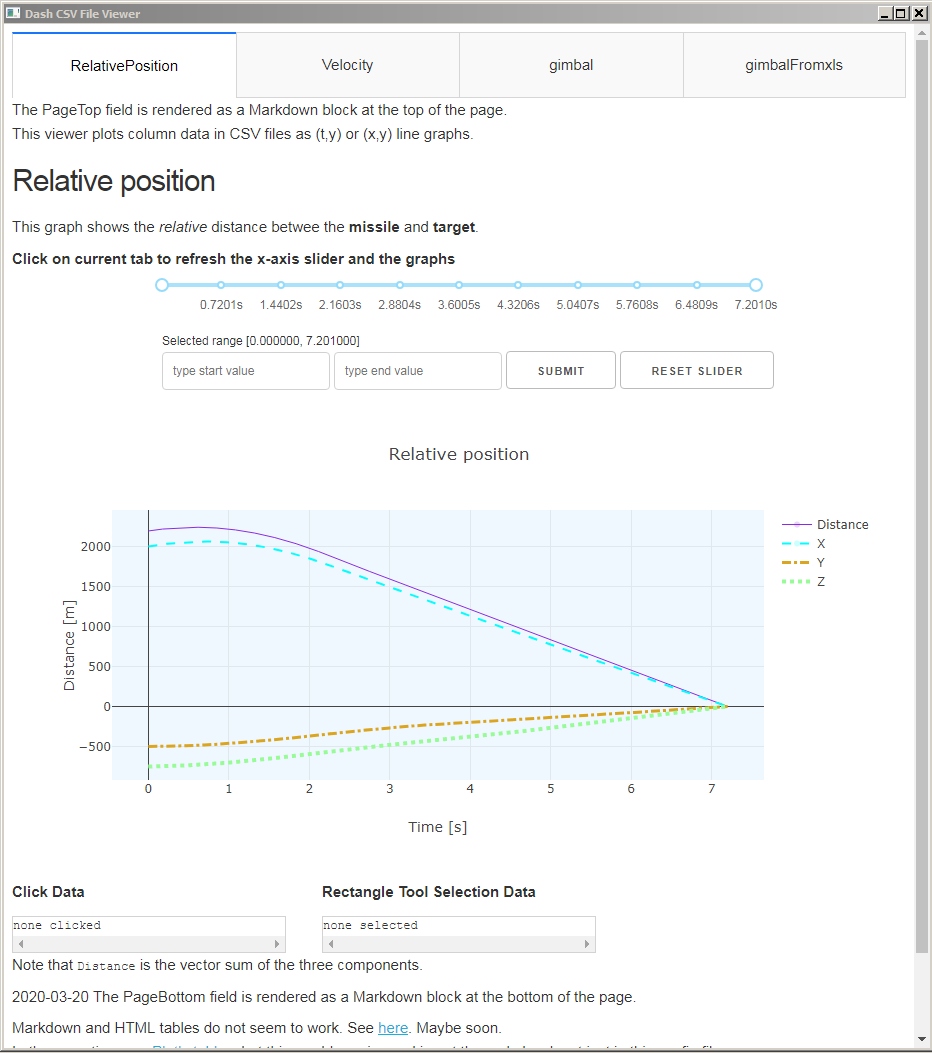
\includegraphics[width=0.70\textwidth]{pic/examplePage}
\caption{Example pages rendered by the dash-lineplot.py utility Python script.
\label{fig:examplePage}}
\end{figure}
 % Introduction

\chapter{Functional Description}

Running the script triggers the creation of a window with one central web browser widget.
The web browser widget is defined to have one page to be rendered on \ac{URL}:

 \url{http://127.0.0.1:8050}.

The page is constructed as an \ac{HTML} page with tagged divisions.
The \ac{HTML} \texttt{<Div>} tag is used to make divisions of content in the web page, e.g. images, header, footer.

A Dash portal is created where the \ac{HTML} page is served via a Flask server.
Dash is a productive Python framework for building web applications.
Written on top of Flask, Plotly.js, and React.js, Dash is ideal for building data visualization applications with highly custom user interfaces in pure Python.

Dash starts a Flask server at the specified \ac{URL}.
The server is started on a daemon thread, i.e. it will run in the background until the main application is terminated.
This means that once the server is running, the page can be viewed in the Dash window as used in this application, or in an external browser.
After the user closed the Dash window, the \ac{URL} can be typed in any web browser to view the current graph set rendered on the \ac{HTML} page.

This page has several elements, all constructed from the information provided in the configuration file. If the user changes the graph definition in the configuration file, the updated page will only be rendered when the script is executed again.

The utility is configured by data entered in an Excel data file. 
The configuration file has any number of sheets where each sheet defines
a different set of line graphs to be rendered on a separate tab in the graph page
(except for the header sheet, which defines the page header.)
The name of the graph sheets in the file always starts with \texttt{graph-} to serve as an identification to the script.
Each graph sheet defines the height of the graphs, axes labels,
one x-value column name and any number of sets of y-value column names.
The graph sets can be rendered each one as a separate figure on the page, or in the subplot format.
Each line has a number of attributes with default values if not supplied.
The tabs on the page can be switched on/off for display purposes.
Each active graph set can also be exported to an interactive \ac{HTML} file for later perusal.

Data from the following file types can be displayed:
\begin{itemize}
  \item \ac{csv} files with column names provided in the first row,
  \item first sheet of an Excel data file with column names provided in the first row,
  \item Matlab format file with data in 'DATA', variable names in 'NAM' and time base in 'TIME'.
\end{itemize}

For more detail on the user level interaction, see Chapter~\ref{chap:userLevelDescription}.
 % Functional Description
\chapter{Input and Output Data}
\label{chap:inputoutput}

The script requires the following input data and folders:


\begin{description}
  \item[configuration file] Excel file with configuration data for the graphing utility.
  \item[./assets] This folder houses the \ac{css} file used to format the contents of the graphing utility (by default, Dash is un-styled). It contains customized, global properties for how to display the \ac{HTML} elements. \ac{css} files can define the size, colour, font, line spacing, indentation, borders, and location of \ac{HTML} elements. An adapted style file from \url{https://codepen.io/chriddyp/pen/bWLwgP} is used.
  \item[./icons] The icons of the various licenses of modules used are stored in this folder.
  \item[./data] Optional data folder. The configuration file can be set up to read from several data files. This folder is used to store the demonstration test set of data files.
\end{description}

The \textbf{graphs} folder is created by the application, if it does not exist.
Interactive \ac{HTML} output graphs from the graphing utility are stored in this folder. Clicking on file, the graph in opened in a browser and full interactive Plotly functionality is available.

 % Input and Output Data
\chapter{Operating System, Licenses and Major Software Versions}


\section{Minimum Requirements}
\label{sec:minReq}

The software requires a 64-bit computer with either Windows 7 or 10 as operating system. If the script is used as a packaged executable, no Python distribution is required. These users can ignore Sections~\ref{sec:requirements},  \ref{sec:softwaredev} and \ref{sec:pyinstaller}.
Software developers and advanced users working with the script code base need to take note of the requirements discussed in these sections.


\section{Licences}
\label{sec:licenses}

The \texttt{dash-lineplot.py} script uses only open source Python modules. The following licenses are applicable:

\begin{itemize}

  \item Python, scipy, numpy, pandas, and other 'standard' modules are licensed under the open source \ac{PSFL}.
  \item Dash and visdcc are released under the permissive \ac{MIT} license.
  \item PySide and Ot are released under the \ac{LGPL}. Note that PyQt5 is not used due to stricter licensing conditions.
  \item PyInstaller is distributed under the \ac{GPL}. This software is not distributed to a client, i.e. only used to package the application.
\end{itemize}

\section{Requirements for Software Developers and Python Script Users}
\label{sec:requirements}

Software required for developers and users working with the code base:

\begin{itemize}
  \item Python 3.7. The preferred distribution is Anaconda 4.7 or higher.
  \item Python modules not included in the Anaconda distribution:
  \begin{itemize}
  \item PySide (Python Qt bindings) with major version 2 on Python 3.7.
  \item Dash visualisation framework with major version 1.
  \item visdcc (run javascript with module Run\_js) version 0.0.40.
  \item PyInstaller, bundles a Python application and its dependencies into a single package, version 3.5.
  \end{itemize}
\end{itemize}


\section{Preparing the Software Developer Environment}
\label{sec:softwaredev}

A personal computer with the minimum requirements listed in Section~\ref{sec:minReq} is required. Install the required software listed in the rest of this section.
Obtain the \texttt{dash-lineplot.py} code and data from the relevant \ac{svn} repository.

\subsection{Installing Anaconda}

Anaconda is a free open-source distribution of Python that aims to simplify package management and deployment. Package versions are managed by the package management system \textsl{conda}.

Obtain the latest version of Anaconda from:

\url{https://www.anaconda.com/distribution/}


When installing Anaconda you are given the option to install for all users or for my user only.  Installing for all users seems to require admin rights when updating or installing packages. It seems that installing for my user has less such issues.  If you find 'write permission' problems, try performing the task using Admin rights.


It is preferred to have the Anaconda/Python paths permanently in the system PATH environment variable. This enables you to open Python from any command window, without using the Anaconda menus settings (When using the Anaconda menu, the paths are set for the one command window instance only).
To enforce this option, ensure that you tick the box on the Anaconda install \ac{GUI} that adds the paths to the Anaconda installation. A convenient Windows tool to inspect the path variables is \url{https://www.rapidee.com/en/about}.

Some installations had difficulty finding the required version of  `libiomp5md.dll`. It appears that one installation (using  \lstinline{Anaconda3-2019.07-Windows-x86_64.exe}) had two (different?) versions of the file:

\footnotesize
\begin{lstlisting}
    where libiomp5md.dll
    C:\ProgramData\Continuum\anaconda3\Library\bin\libiomp5md.dll
    C:\Program Files (x86)\Common Files\Intel\Shared Files\cpp\Bin\Intel64\\libiomp5md.dll
\end{lstlisting}
\normalsize
Make sure that the Anaconda path comes first, above the other instances.  Note that this may break the other application using the other instance.

\subsection{Installing Python Packages not included in Anaconda}

\textit{conda-forge} is a community effort that provides \textit{conda} packages not included in Anaconda. Registration of the \textit{conda-forge} channel as a package source for \textit{conda} might be required.

\footnotesize
\begin{lstlisting}
    conda config --add channels conda-forge
\end{lstlisting}
\normalsize

Install the required packages not included in the Anaconda distribution from a Windows Console:
\footnotesize
\begin{lstlisting}
    conda update conda

    conda install -c conda-forge dash
    conda install -c conda-forge pyside2
    conda install -c conda-forge pyinstaller
    conda install -c conda-forge visdcc

\end{lstlisting}
\normalsize

Online installation of additional packages, as well as updates to the Anaconda distribution is preferred.
A recent off-line install required the following packages to be manually installed.

\footnotesize
\begin{lstlisting}
    conda install dash-0.39.0-py_0.tar.bz2
    conda install flask-compress-1.4.0-py_0.tar.bz2
    conda install plotly-4.1.1-py_0.tar.bz2
    conda install dash-html-components-0.14.0-py_0.tar.bz2
    conda install dash-core-components-0.44.0-py_0.tar.bz2
    conda install dash-table-3.6.0-py_0.tar.bz2
    conda install dash-daq-0.1.4-py_0.tar.bz2
    conda install plotly-orca-1.2.1-1.tar.bz2
    conda install retrying-1.3.3-py37_1.tar.bz2
    conda install dash-renderer-0.20.0-py_0.tar.bz2
    conda install visdcc-0.0.40-pyh516909a_0.tar.bz2
    conda install pyside2-5.13.1-py37hfa7ce6d_6.tar.bz2

\end{lstlisting}
\normalsize

Install PyInstaller only if final packaging of the application is required.

\subsection{Developer Software Tools}

\label{sec:devtools}

A software version control system provides a centralised storage and management of the code base and supporting data files.
It keeps track of all changes and allows recovery of previous versions of the code and data.
The software and supporting data files are under the \ac{OSSIM}  \ac{svn} \ac{SVC} at \ac{URL}:

\footnotesize
\url{svn://localhost/cms/trunk/green/red/user/tools/python/dash-lineplot}
\normalsize

The Windows \ac{GUI} client TortoiseSVN, available from

\url{https://tortoisesvn.net/downloads.html}

is recommended. It's intuitive and easy to use, since it doesn't require the \ac{svn} command line client to run. It is free to use, even in a commercial environment. If you prefer hands-on command line \ac{svn} interaction, tick the command line client installation box during installation.

Any text editor can be used to edit the Python code. \ac{VS} Code is a lightweight but powerful source code editor which runs on your desktop and is available for Windows, macOS and Linux. It comes with built-in support for JavaScript, TypeScript and Node.js and has a rich ecosystem of extensions for other languages (such as C++, C\#, Java, Python, PHP, Go) and runtimes (such as .NET and Unity). Download \ac{VS} Code from

\url{https://code.visualstudio.com/}

This document was generated using the \LaTeX{} typesetting system. It is recommended that the MikTeX distribution be used on Windows. Download from \url{www.miktex.org} or from the \ac{TUG} web site at \url{https://tug.org/}. Suitable specialised editing tools include WinEdt (commercial but inexpensive) at \url{www.winedt.com}, or use \ac{VS} Code as \ac{IDE}.


\section{Packaging for User Distribution}
\label{sec:pyinstaller}

PyInstaller reads a Python script and analyses the code to discover every other module and library the script needs in order to execute.
It finds the imported modules and looks in them for \textit{import} statements, and so on recursively, until it has a complete list of modules the script may use.
Some Python scripts import modules in ways that PyInstaller cannot detect. If the script requires files that PyInstaller does not know about, it can be specified in various ways:

\begin{itemize}
  \item Specify additional files on the command line.
  \item Specify additional import paths on the command line.
  \item Modify the \texttt{spec} file created by PyInstaller.
\end{itemize}

After analyses, it collects copies of all the files, including the active Python interpreter, and puts them with the script in a single folder, or optionally in a single executable file.

The bundled application does not include any source code. PyInstaller bundles compiled Python scripts (\texttt{.pyc} files). These could in principle be decompiled to reveal the logic of the code.
Python byte code can be obfuscated with AES256 by specifying an encryption key on PyInstaller's command line.

On the first run of PyInstaller, with the main script as input parameter, a \texttt{spec} file, with the same name as the input script, is generated.

\footnotesize
\begin{lstlisting}
    pyinstaller options myscript.py
\end{lstlisting}
\normalsize

The \texttt{spec} file tells PyInstaller how to process the script. It encodes the script names and command line options provided to the PyInstaller command. The \texttt{spec} file is actually executable Python code. PyInstaller builds the bundled application by executing the contents of the \texttt{spec} file.

There are certain cases where it is useful to modify the \texttt{spec} file:

\begin{itemize}
  \item When you want to bundle data files with the application.
  \item When you want to include run-time libraries (.dll or .so files) that PyInstaller does not know about from any other source.
  \item When you want to add Python run-time options to the executable.
  \item When you want to create a multiprogram bundle with merged common modules.
\end{itemize}


For more on this topic, see \url{https://pyinstaller.readthedocs.io/en/stable/spec-files.html}.

\subsection{Bundling to a single folder}
\label{sec:bundledFolder}

Initial usage, bundling to a folder, resulted in the first \texttt{dash-lineplot.spec} file:

\footnotesize
\begin{lstlisting}
    pyinstaller dash-lineplot.py
\end{lstlisting}
\normalsize

Data files and folders required by the script are added in the \texttt{spec} file, see the \texttt{added\_files} list in the listing below. It was necessary to use local copies of the following packages used in the application: \texttt{platforms, dash, plotly, visdcc} and some \texttt{qt} packages related to the \texttt{QtWebEngineProcess} used in the graphing display. These packages are included in the \texttt{pyInstaller} folder in the application source tree.

An example \texttt{spec} file for the \texttt{dash-lineplot.py} script:

\footnotesize
\begin{lstlisting}

    block_cipher = None

    added_files = [
             ( 'icons', 'icons' ),
             ( 'assets', 'assets'),
             ( 'data', 'data'),
             ( 'dash-config.xlsx', '.'),
             ( 'pyInstaller\\platforms', 'platforms' ),
             ( 'pyInstaller\\dash\\dash_core_components', 'dash_core_components'),
             ( 'pyInstaller\\dash\\dash_html_components', 'dash_html_components'),
             ( 'pyInstaller\\dash\\dash_renderer', 'dash_renderer'),
             ( 'pyInstaller\\dash\\dash', 'dash'),
             ( 'pyInstaller\\plotly', 'plotly'),
             ( 'pyInstaller\\qt\\translations', 'translations'),
             ( 'pyInstaller\\qt\\resources', 'resources'),
             ( 'pyInstaller\\qt\\qt.conf', '.'),
             ( 'pyInstaller\\qt\\QtWebEngineProcess.exe', '.'),
             ( 'pyInstaller\\visdcc', 'visdcc'),
             ( 'pyInstaller\\startPlotTool.bat', '.'),
             ]

    a = Analysis(['dash-lineplot.py'],
                 pathex=['C:\\Temp'],
                 datas=added_files,
                 hiddenimports=['PyQt5.QtWebEngineWidgets','PyQt5.QtNetwork',
                 'PyQt5.QtWebEngineCore', 'PyQt5.QtWebChannel','PyQt5.QtPrintSupport'],
                 hookspath=[],
                 runtime_hooks=[],
                 excludes=['tkinter'],
                 win_no_prefer_redirects=False,
                 win_private_assemblies=False,
                 cipher=block_cipher,
                 noarchive=False)
    pyz = PYZ(a.pure, a.zipped_data,
                 cipher=block_cipher)
    exe = EXE(pyz,
              a.scripts,
              [],
              exclude_binaries=True,
              name='dash-lineplot',
              debug=False,
              bootloader_ignore_signals=False,
              strip=False,
              upx=True,
              console=True )
    coll = COLLECT(exe,
                   a.binaries,
                   a.zipfiles,
                   a.datas,
                   strip=False,
                   upx=True,
                   upx_exclude=[],
                   name='dash-lineplot')


\end{lstlisting}
\normalsize

Bundled to a folder, PyInstaller creates a folder with the same name as the main Python script. This folder contains all the script dependencies, an executable file named after the Python script and any files or folders required by the script specified in the \texttt{spec} file.

Experimentation with PyInstaller showed that there might be a second copy of the \texttt{QtWebEngineProcess} executable in a folder \url{dist/dash-lineplot/PyQt5/Qt/bin/}. Removing this file ensures correct operation. A batch script \texttt{runPyInstaller.bat}, is available in the application top level folder for packaging of the application:

\footnotesize
\begin{lstlisting}
    @echo off

    pyInstaller dash-lineplot.spec

    echo .
    echo .
    echo Removing QtWebEngineProcess.exe from the PyQt5\Qt\bin\ path if present.
    echo .

    del dist\dash-lineplot\PyQt5\Qt\bin\QtWebEngineProcess.exe

    set /p DUMMY=done, hit ENTER to exit

\end{lstlisting}
\normalsize


Running this script in a folder named \texttt{lineplot} results in the folder structure depicted in Figure~\ref{fig:folderdist}. Note that the distribution folder is inside the \texttt{dist} folder.


\begin{figure}[h]
\centering
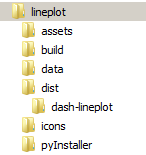
\includegraphics[width=0.3\textwidth]{pic/folderDist}
\caption{Folder structure in bundling \texttt{dash-lineplot.py} with PyInstaller to a distribution folder.
\label{fig:folderdist}}
\end{figure}


The \texttt{dash-lineplot} folder can now be compressed to \texttt{dash-lineplot.zip} and transmitted to the user computer. Installation on the user computer is a simple unzip of the \texttt{zip} file. The user runs the application by opening the folder and launching the \texttt{dash-lineplot} executable by running the \texttt{startPlotTool.bat} script in the top-level folder:

\footnotesize
\begin{lstlisting}
    @echo off

    echo Starting the Dash Line Plot Graphing Tool ....
    echo.
    echo.

    cd dash-lineplot

    if [%1]==[] dash-lineplot.exe
    if not [%1]==[] dash-lineplot.exe --configfile=%1

    set /p DUMMY=done, hit ENTER to exit
\end{lstlisting}
\normalsize

\subsection{Bundling to a single file}

The code can also be bundled to one file:

\footnotesize
\begin{lstlisting}
    pyinstaller --onefile dash-lineplot.py
\end{lstlisting}
\normalsize

In this case \texttt{dash-lineplot.py} script and all its dependencies are bundled into a single executable
named \texttt{dash-lineplot.exe}. One single (very large!) file is distributed to the client.  When started it creates a temporary folder in the appropriate temp-folder location for the operating system. The folder is named \texttt{\_MEIxxxxxx}, where \texttt{xxxxxx} is a random number. The boot loader uncompresses the support files and writes copies into the temporary folder. This can take a little time. That is why a one-file application distribution is slower to start than a one-folder distribution. After creating the temporary folder, the boot loader proceeds exactly
as for the one-folder bundle, in the context of the temporary folder. When the bundled code terminates,
the boot loader deletes the temporary folder.


 % Operating System, Major Software Versions and Licenses


\chapter{User-level Description}

\label{chap:userLevelDescription}
\section{Starting the Dash Line Plot Graphing Utility}


The application is distributed

\begin{itemize}
  \item either as a Python script, i.e. \texttt{dash-lineplot.py},
  \item or as an executable file, i.e. \texttt{dash-lineplot.exe}.
\end{itemize}

Double-clicking on any one of these files will start the application.
If the computer is not set up to associate \texttt{.py} files with the Python interpreter, open a windows command prompt window and type the following:

\footnotesize
\begin{lstlisting}
  python dash-lineplot.py
\end{lstlisting}
\normalsize

Working in a command prompt window is recommended. Warning and error messages output to the screen are published to the console. This can aid in tracing unexpected errors.

Working in an environment where the script was packaged to an executable, start the application from a console by typing

\footnotesize
\begin{lstlisting}
  dash-lineplot.exe
\end{lstlisting}
\normalsize

An easy, and recommended way of opening a command prompt at the correct folder location, is by following the steps:

\begin{itemize}
  \item Open the File Explorer.
  \item Navigate to the folder where the application Python script or executable is housed.
  \item Click in die File Explorer address bar.
  \item Type \texttt{cmd} into the address bar.
  \item Hit enter.
\end{itemize}

Hint: See 
\footnotesize
\url{https://www.howtogeek.com/235101/10-ways-to-open-the-command-prompt-in-windows-10/} \normalsize
for other ways to open a command prompt on Windows 10.

For ease of use a Windows batch script, \texttt{startPlotTool.bat}, is available in both environments. This script simply encapsulates the above commands:

\footnotesize
\begin{lstlisting}
    @echo off

    echo Starting the Dash Line Plot Graphing Tool ...
    echo.
    echo.

    if [%1]==[] python dash-lineplot.py
    if not [%1]==[] python dash-lineplot.py --configfile=%1

    set /p DUMMY=done, hit ENTER to exit
\end{lstlisting}
\normalsize

or

\footnotesize
\begin{lstlisting}
    @echo off

    echo Starting the Dash Line Plot Graphing Tool ....
    echo.
    echo.

    cd dash-lineplot

    if [%1]==[] dash-lineplot.exe
    if not [%1]==[] dash-lineplot.exe --configfile=%1

    set /p DUMMY=done, hit ENTER to exit
\end{lstlisting}
\normalsize


Starting the script with no commandline arguments results in loading the default \texttt{dash-config.xlsx} configuration file. A configuration file name can be specified on the commandline, using any of the following options:

\footnotesize
\begin{lstlisting}
  python dash-lineplot.py --configfile=anotherFileName.xlsx

  dash-lineplot.exe --configfile=anotherFileName.xlsx
  
  startPlotTool.bat anotherFileName.xlsx

\end{lstlisting}
\normalsize

Note that using the packaged version, the batch file starting the application is distributed at one folder level up from the actual distribution. This is done to give easy access to the script. The configuration file must be specified relative to the actual distribution folder. Figure~\ref{fig:folderdistEx} shows the position of the startup script relative to the distribution folder. In the script the directory is changed to the \texttt{dash-lineplot} folder and only then is the executable started. The configuration file is therefore always found on the path relative to folder \texttt{dash-lineplot}.

\begin{figure}[h]
\centering
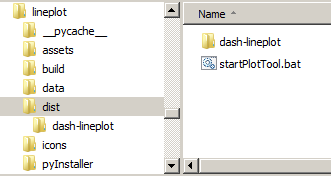
\includegraphics[width=0.5\textwidth]{pic/folderDistEx}
\caption{Distribution folder structure showing the location of the startup batch script.
\label{fig:folderdistEx}}
\end{figure}


\section{Setup and Usage}


\subsection{Configuration File and Page Layout}

Figures~\ref{fig:dashviewConfig1} and \ref{fig:dashviewConfig2} show the documentation sheet of the Excel plotting configuration file. A short description of variables are provided on this sheet. Refer to the information presented in these figures, no further details are provided in this document.

\begin{figure}[h]
\centering
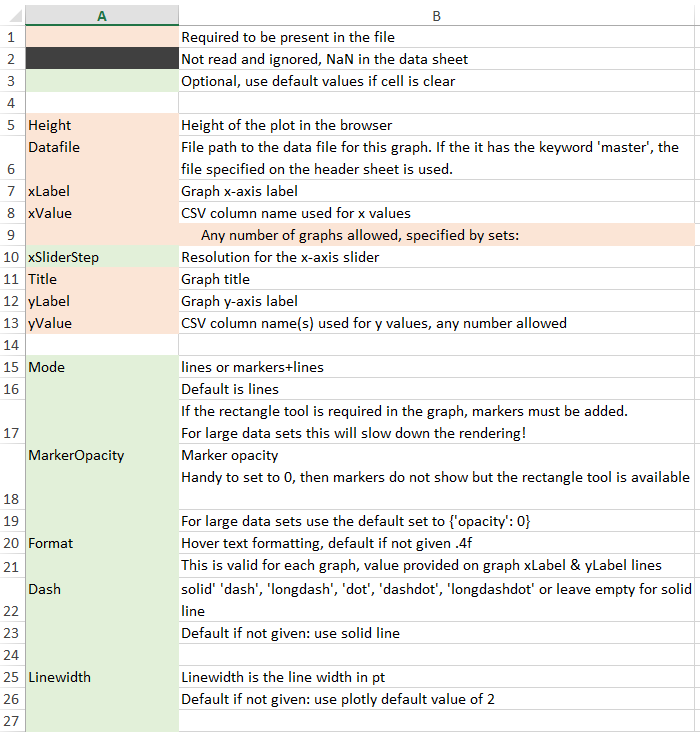
\includegraphics[width=0.90\textwidth]{pic/dashview-config1}
\caption{Documentation sheet of the Excel plotting configuration file.
\label{fig:dashviewConfig1}}
\end{figure}

\begin{figure}[h]
\centering
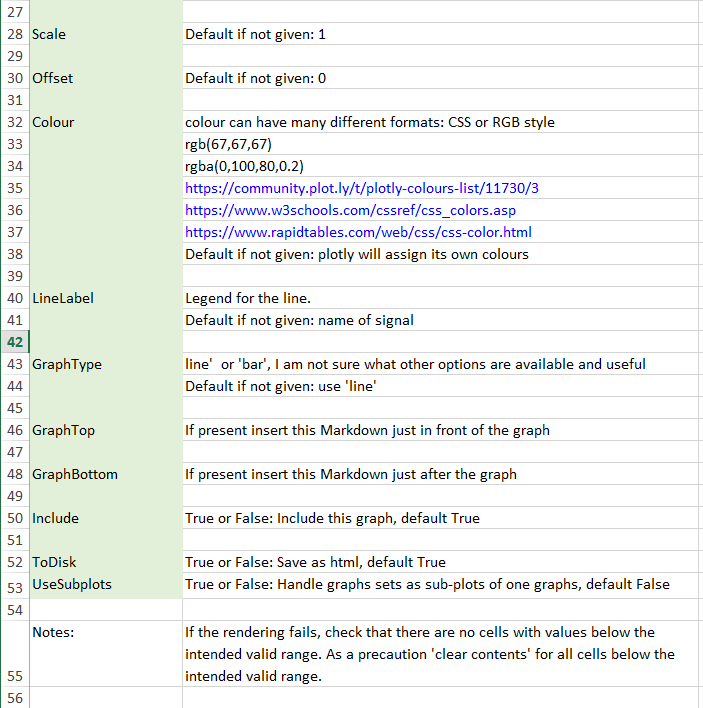
\includegraphics[width=0.90\textwidth]{pic/dashview-config2}
\caption{Documentation sheet of the Excel plotting configuration file (continued).
\label{fig:dashviewConfig2}}
\end{figure}

The header sheet in the configuration file, see annotated Figure~\ref{fig:dashview-config-header}, provides general information published on each page of the display. The user can provide a data file name on this sheet for general use. Sheets can refer to this file with the keyword \texttt{master} in the \texttt{Datafile} \texttt{Value} entry.

\begin{figure}[h]
\centering
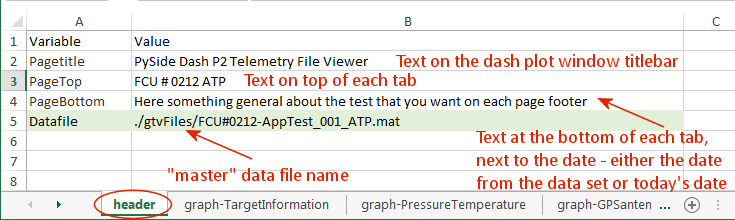
\includegraphics[width=0.90\textwidth]{pic/dashview-config-header}
\caption{Header sheet in the configuration file.
\label{fig:dashview-config-header}}
\end{figure}

Figures~\ref{fig:dashview-config-oscPL45} and \ref{fig:dashview-config-imuRates} are two example setup sheets specifying data configuration for plotting. The setup shown in Figure~\ref{fig:dashview-config-oscPL45} results in each set of traces to be plotted on a separate Plotly figure. The setup in Figure~\ref{fig:dashview-config-imuRates} makes use of Plotly subplots. Using subplots enables hover data on traces to be displayed simultaneously for all traces defined on the sheet, see example in Figure~\ref{fig:dashview-imuRates}. Exactly the same graph set plotted without the use of subplot is shown in Figure~\ref{fig:dashview-config-imuRates-noSubplots}.

\begin{figure}[h]
\centering
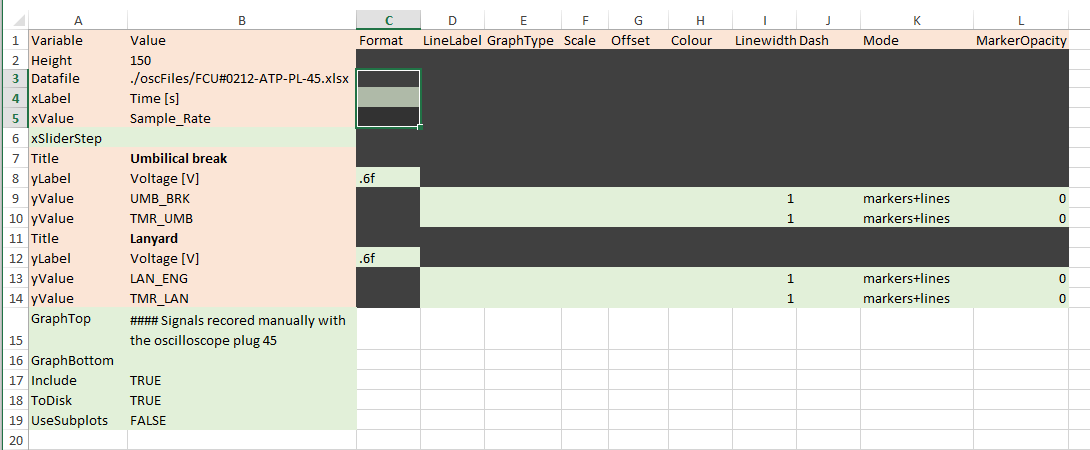
\includegraphics[width=\textwidth]{pic/dashview-config-oscPL45}
\caption{Example graph setup where subplots are not used, transparent markers are used and hover data format is specified.
\label{fig:dashview-config-oscPL45}}
\end{figure}
\begin{figure}[h]
\centering
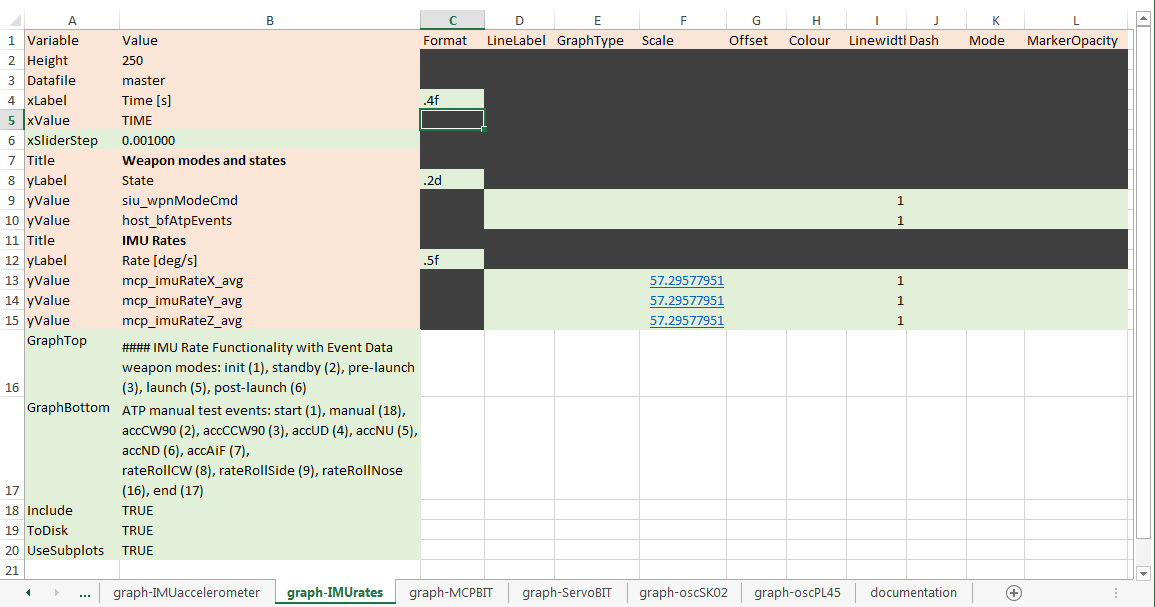
\includegraphics[width=\textwidth]{pic/dashview-config-imuRates}
\caption{Example setup where subplots are used, the IMU rates are scaled, no markers are used and hover data format is specified.
\label{fig:dashview-config-imuRates}}
\end{figure}

Figure~\ref{fig:dashview-imuRates} links the entries in the configuration file (refer to Figure~\ref{fig:dashview-config-imuRates}) to the format of the graph page. Note the following:

\begin{itemize}
  \item The tab name corresponds to the sheet name in the configuration file, omitting the leading \texttt{graph-} phrase.
  \item The header and footer at the top and bottom of the page are from the \texttt{header} sheet.
  \item The text entries just below and above these are the \texttt{GraphTop} and \texttt{GraphBottom} \texttt{Value} entries on the sheet.
  \item Two sets of traces are defined on the sheet, using subplots. Usage of the subplot option enables hover data to be displayed on all traces simultaneously.
  \item The hover data format is specified for the x-axis and two y-axis separately.
  \item The subplot titles, y-axis and x-axis labels are as provided in the \texttt{graph-IMUrates} sheet of the configuration file.
\end{itemize}

The same data is displayed in Figure~\ref{fig:dashview-config-imuRates-noSubplots}, not using the subplot functionality.

\begin{figure}[h]
\centering
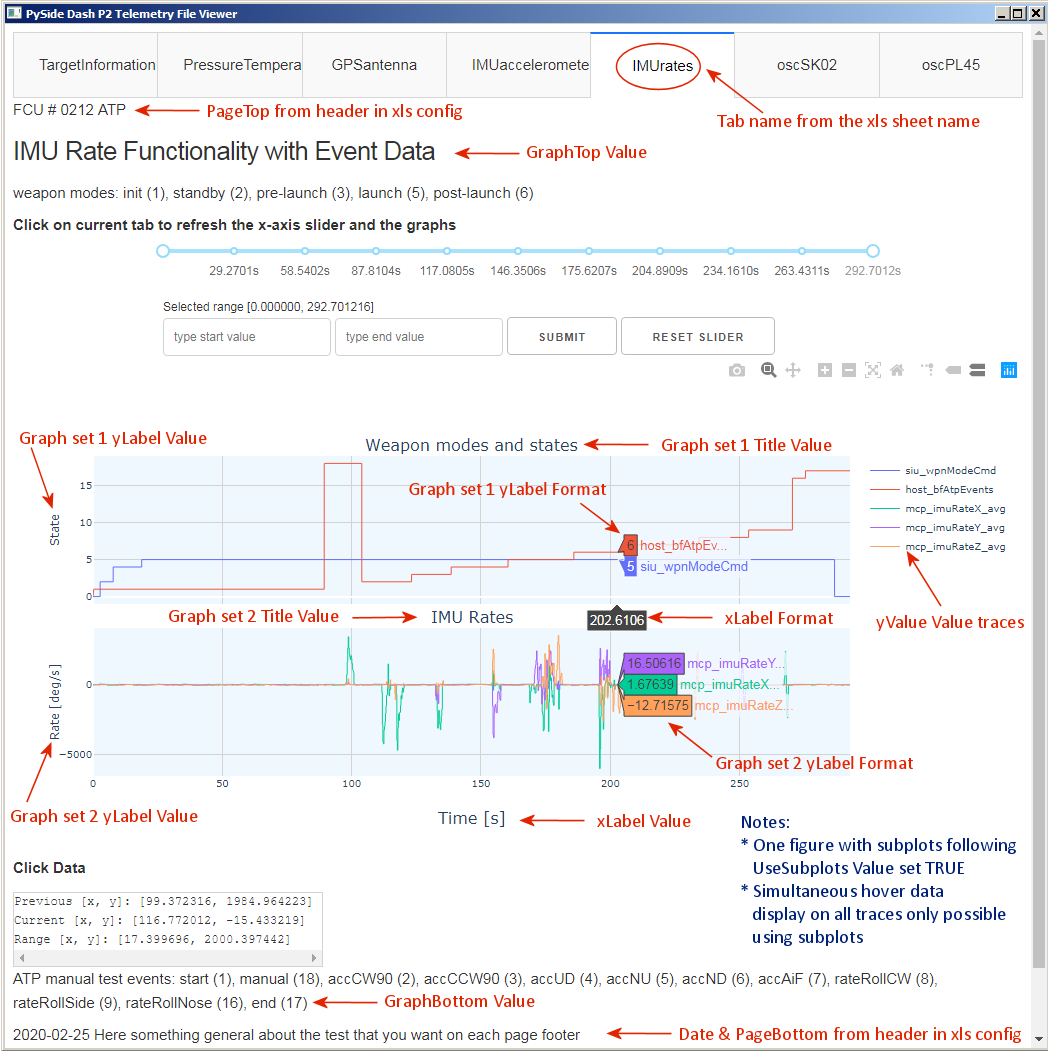
\includegraphics[width=\textwidth]{pic/dashview-imuRates}
\caption{Plot tab the IMU rates graph setup example, using subplots.
\label{fig:dashview-imuRates}}
\end{figure}


\begin{figure}[h]
\centering
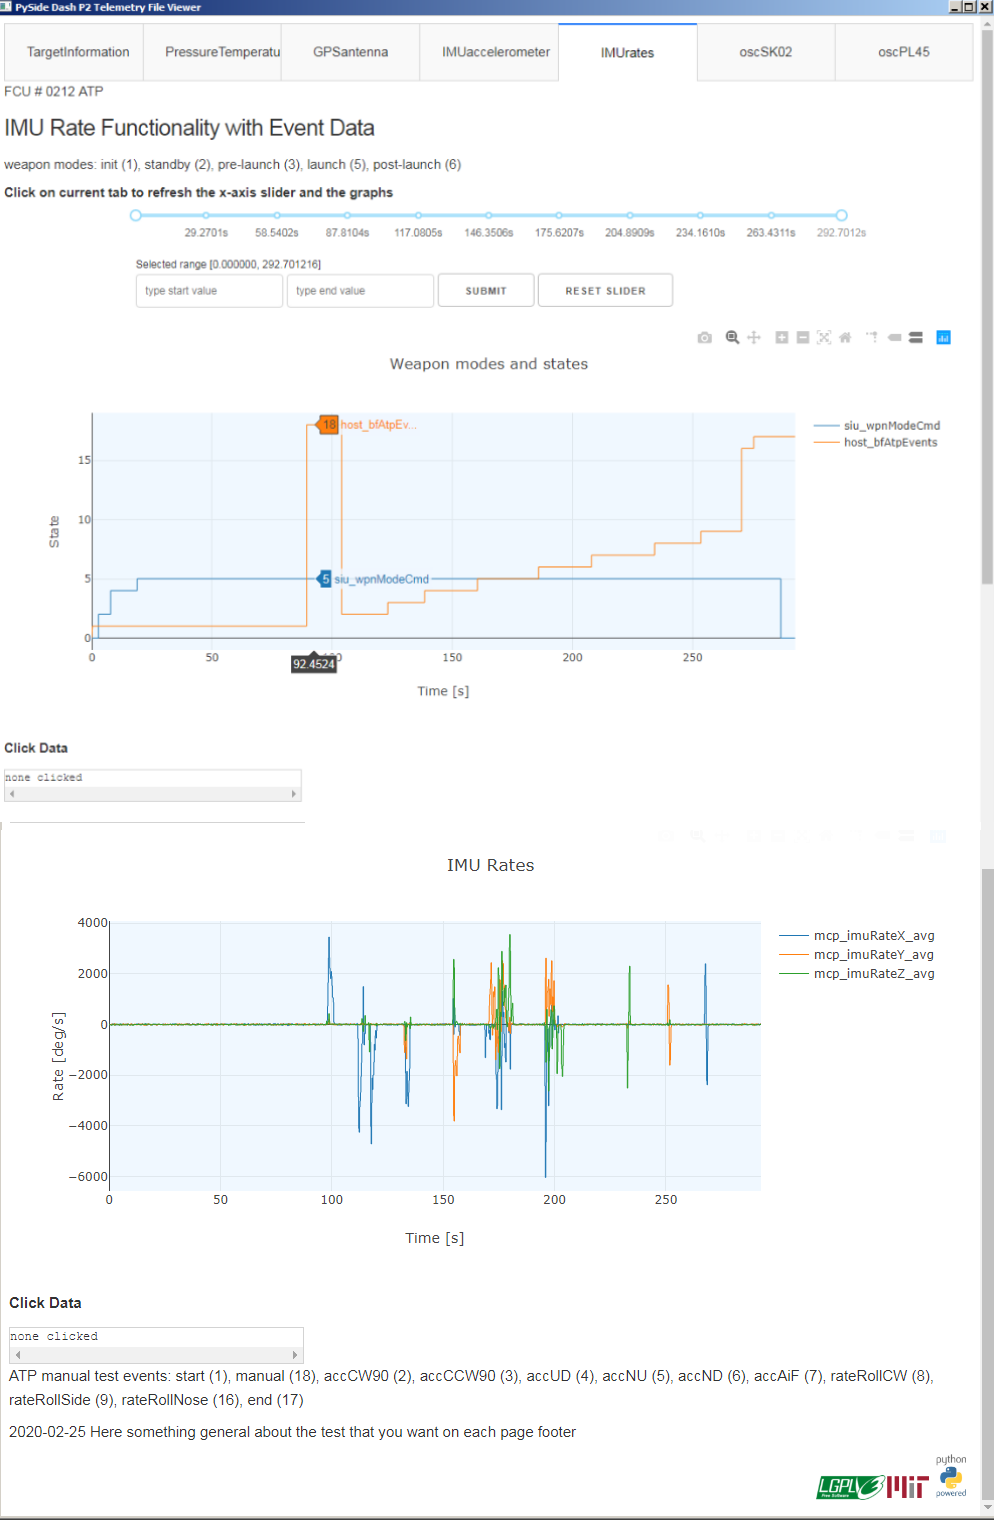
\includegraphics[height=0.95\textheight]{pic/dashview-config-imuRates-noSubplots}
\caption{Plot tab the IMU rates graph setup example, not using subplots.
\label{fig:dashview-config-imuRates-noSubplots}}
\end{figure}

\clearpage
\subsection{Slider Usage}

An x-axis slider is available at the top of each page, covering the data set x-axis data range. Refer to Figure~\ref{fig:dashview-subPlot2Slider1}. The user sets the minimum and maximum value of the x-axis with the slider handles. The text box immediately displays the selected range. The increments at which the slider values change are controlled by the specification from the configuration file. The user however has to click on the current page tab before the graphs are redrawn to display only data in the selected x-axis range, see Figure~\ref{fig:dashview-subPlot2Slider2}. The reset button will reset the x-axis limits to that of the data set.

\begin{figure}[h]
\centering
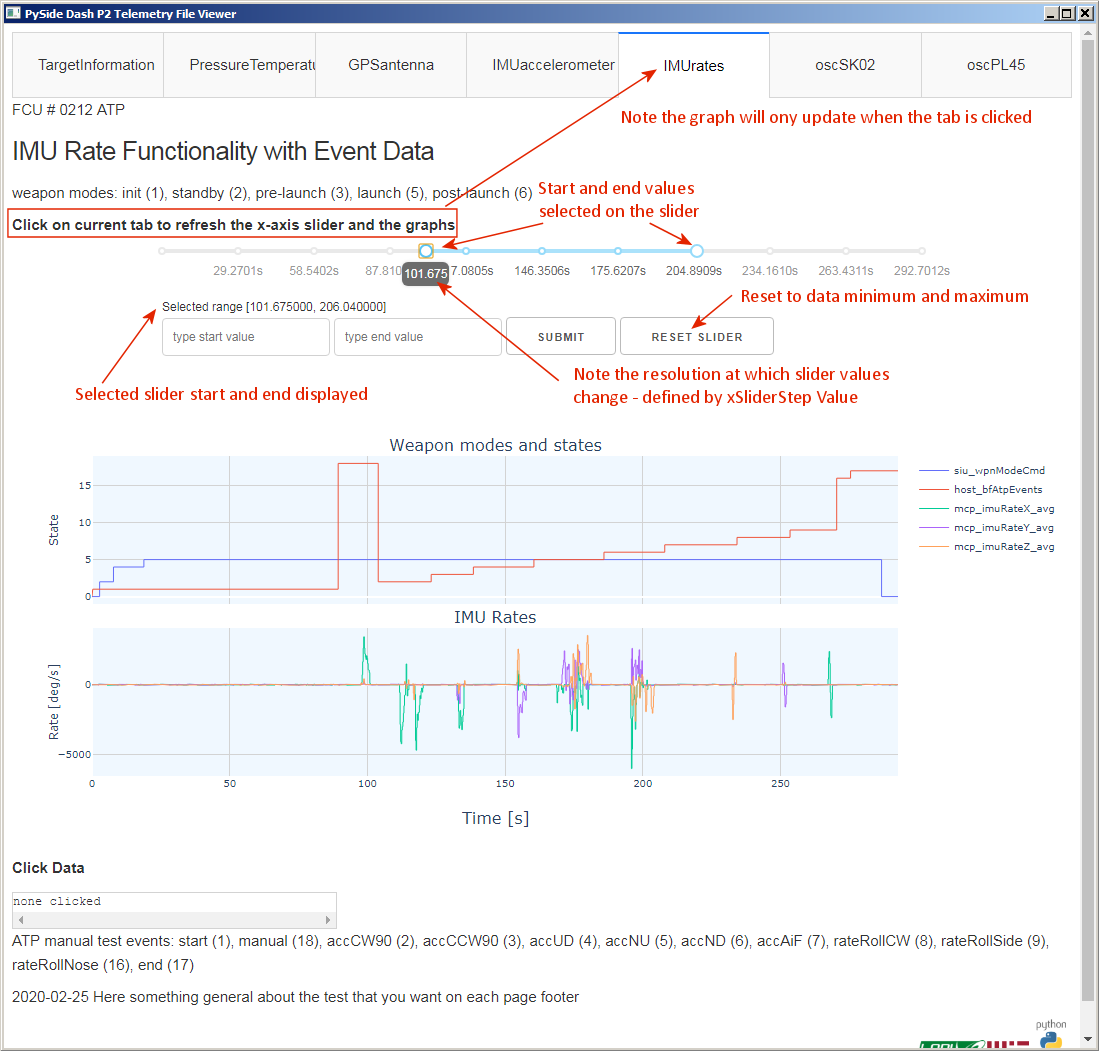
\includegraphics[width=\textwidth]{pic/dashview-subPlot2Slider1}
\caption{The x-axis slider at the top of the page provides the capability to zoom the complete data set to a user selected x-range.
\label{fig:dashview-subPlot2Slider1}}
\end{figure}

\begin{figure}[h]
\centering
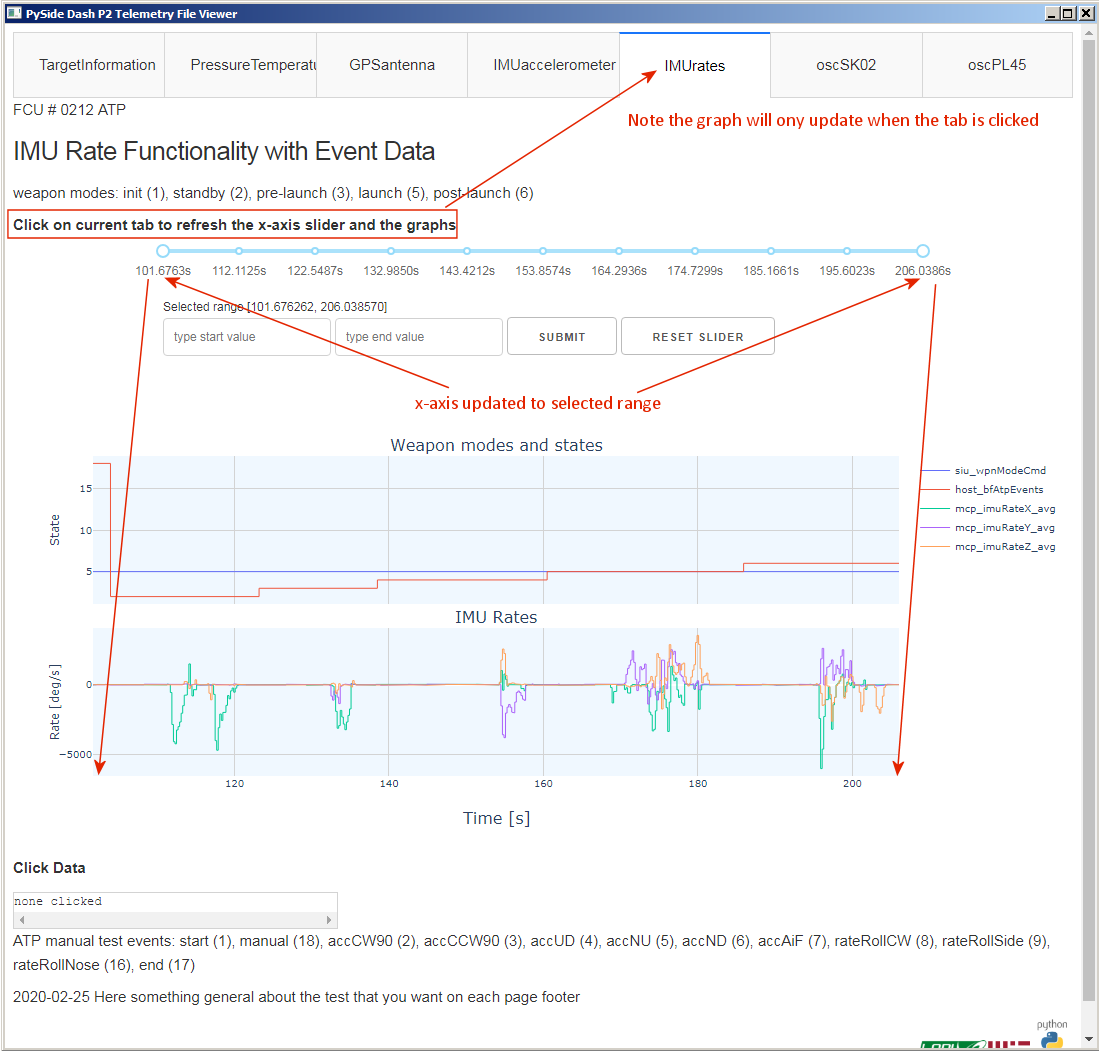
\includegraphics[width=\textwidth]{pic/dashview-subPlot2Slider2}
\caption{A click on the current page tab triggers the redraw of the page, using only data in the x-axis range selected by the user.
\label{fig:dashview-subPlot2Slider2}}
\end{figure}

\clearpage

The x-axis range can also be set by typing values in the text boxes just below the slider. Refer to Figure~\ref{fig:dashview-subPlot2Slider3}. The submit button records these selected values and activates the display of the selected range in the dedicated text box. A click on the tab will trigger an update to the graph data displayed.

\begin{figure}[h]
\centering
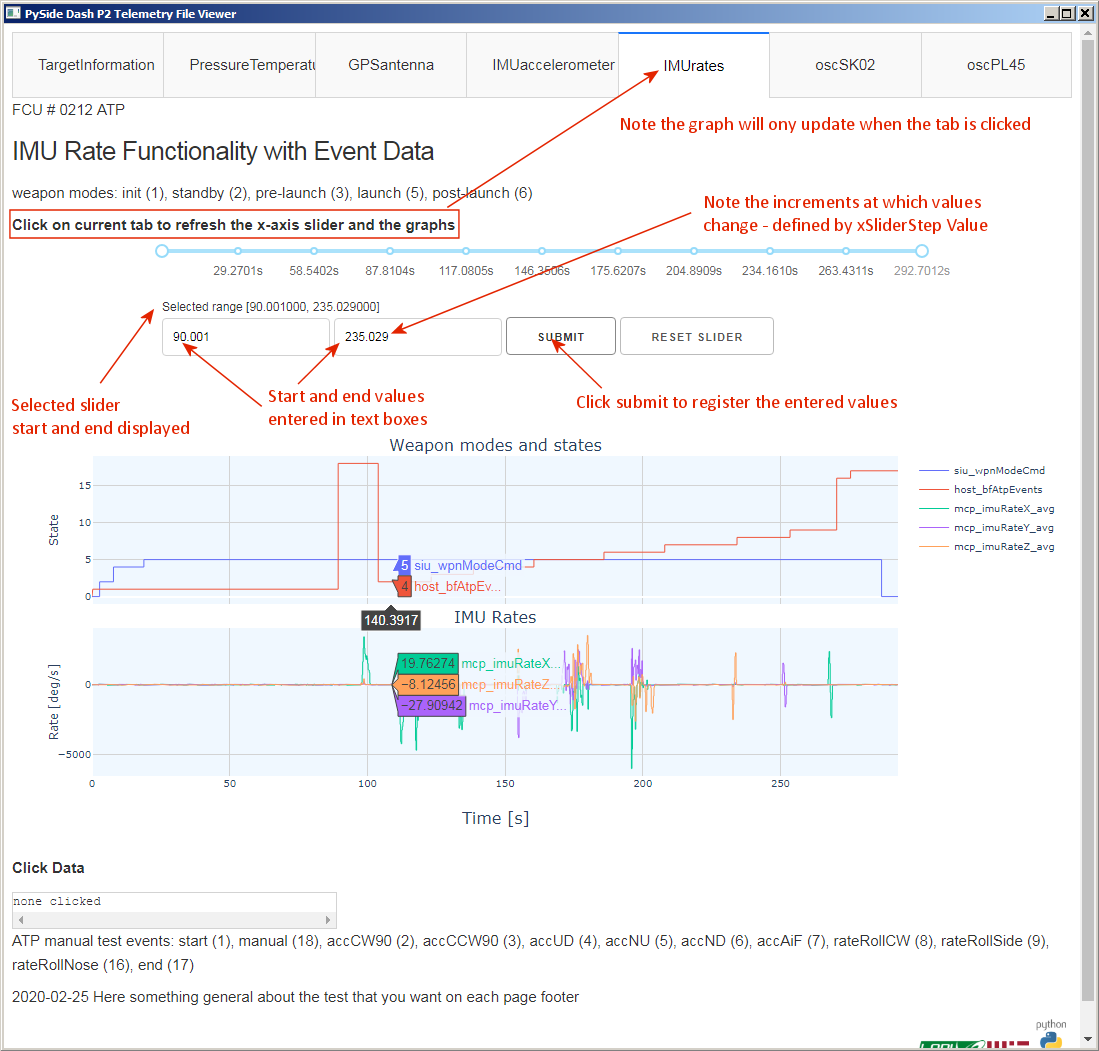
\includegraphics[width=\textwidth]{pic/dashview-subPlot2Slider3}
\caption{The user can specify the start and end values of the x-axis using the text boxes provided. The submit button will register the values for use when redrawing the graphs.
\label{fig:dashview-subPlot2Slider3}}
\end{figure}

\clearpage
\subsection{Range Measurements on Graphs}

Two methods are available to do a measurement on the graphs (see Figure~\ref{fig:dashview-rectangleDataSelect}):
\begin{description}
  \item [Click Data:] The user can click on any trace to record the clicked point in the \texttt{Click Data} box below the relevant graph. When a second data point is clicked, the range in x and y are reflected in the display text box. This functionality is available for individual Plotly figures, as well as subplot figures. The click functionality can be used in conjunction with the standard Plotly zoom functionality.
  \item [Rectangle Tool Selection Data:] The Plotly rectangle tool will only appear in the toolbar of the figure if markers are used for one or more traces in the figure. For large data sets, usage of this tool is not recommended since it slows down the drawing process. If the user prefers to use this tool, the opacity of the markers can be set to 0 in order to not clutter the graph. To measure using the rectangle tool, click on the tool in the toolbar, then draw the rectangle on the graph using the mouse. The top-left, bottom-right and range in x and y are displayed in the \texttt{Rectangle Tool Selection Data} text box to below the relevant graph. This functionality can also be used in conjunction with the Plotly zoom functionality.
\end{description}

\begin{figure}[h]
\centering
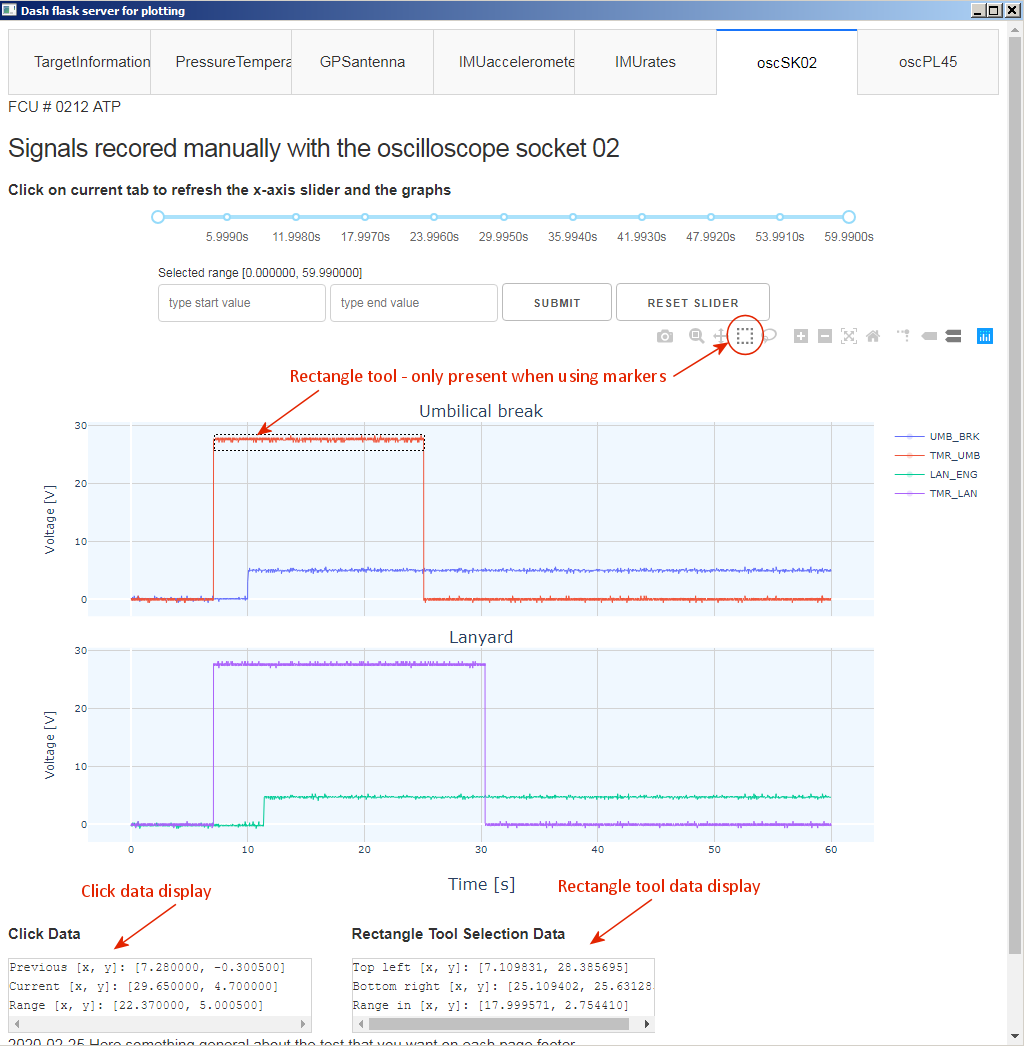
\includegraphics[width=\textwidth]{pic/dashview-rectangleDataSelect}
\caption{Using the Click and Rectangle tools to do measurements on the data set.
\label{fig:dashview-rectangleDataSelect}}
\end{figure}
 % User-level Description


\clearpage

\appendix
\chapter{OPEN SOURCE SOFTWARE LICENSES}
\label{app:licenses}

\section{GPLv3: GNU General Public License}

The PyInstaller is released under this license

\url{https://www.gnu.org/licenses/gpl-3.0.html}:

\scriptsize
\begin{verbatim}

GNU GENERAL PUBLIC LICENSE
Version 3, 29 June 2007

Copyright   2007 Free Software Foundation, Inc. <https://fsf.org/>

Everyone is permitted to copy and distribute verbatim copies of this license
document, but changing it is not allowed.

Preamble
The GNU General Public License is a free, copyleft license for software and
other kinds of works.

The licenses for most software and other practical works are designed to take
away your freedom to share and change the works. By contrast, the GNU General
Public License is intended to guarantee your freedom to share and change all
versions of a program--to make sure it remains free software for all its users.
We, the Free Software Foundation, use the GNU General Public License for most
of our software; it applies also to any other work released this way by its
authors. You can apply it to your programs, too.

When we speak of free software, we are referring to freedom, not price. Our
General Public Licenses are designed to make sure that you have the freedom to
distribute copies of free software (and charge for them if you wish), that you
receive source code or can get it if you want it, that you can change the software
or use pieces of it in new free programs, and that you know you can do these things.

To protect your rights, we need to prevent others from denying you these rights or
asking you to surrender the rights. Therefore, you have certain responsibilities
if you distribute copies of the software, or if you modify it: responsibilities to
respect the freedom of others.

For example, if you distribute copies of such a program, whether gratis or for a
fee, you must pass on to the recipients the same freedoms that you received. You
must make sure that they, too, receive or can get the source code. And you must
show them these terms so they know their rights.

Developers that use the GNU GPL protect your rights with two steps: (1) assert
copyright on the software, and (2) offer you this License giving you legal permission
to copy, distribute and/or modify it.

For the developers' and authors' protection, the GPL clearly explains that there is
no warranty for this free software. For both users' and authors' sake, the GPL
requires that modified versions be marked as changed, so that their problems will
not be attributed erroneously to authors of previous versions.

Some devices are designed to deny users access to install or run modified versions
of the software inside them, although the manufacturer can do so. This is
fundamentally incompatible with the aim of protecting users' freedom to change
the software. The systematic pattern of such abuse occurs in the area of products
for individuals to use, which is precisely where it is most unacceptable.
Therefore, we have designed this version of the GPL to prohibit the practice for
those products. If such problems arise substantially in other domains, we stand
ready to extend this provision to those domains in future versions of the GPL,
as needed to protect the freedom of users.

Finally, every program is threatened constantly by software patents. States should
not allow patents to restrict development and use of software on general-purpose
computers, but in those that do, we wish to avoid the special danger that patents
applied to a free program could make it effectively proprietary. To prevent this,
the GPL assures that patents cannot be used to render the program non-free.

The precise terms and conditions for copying, distribution and modification follow.

TERMS AND CONDITIONS
0. Definitions.
"This License" refers to version 3 of the GNU General Public License.

"Copyright" also means copyright-like laws that apply to other kinds of works,
such as semiconductor masks.

"The Program" refers to any copyrightable work licensed under this License. Each
licensee is addressed as "you". "Licensees" and "recipients" may be individuals or
organizations.

To "modify" a work means to copy from or adapt all or part of the work in a fashion
requiring copyright permission, other than the making of an exact copy. The
resulting work is called a "modified version" of the earlier work or a work
"based on" the earlier work.

A "covered work" means either the unmodified Program or a work based on the Program.

To "propagate" a work means to do anything with it that, without permission, would
make you directly or secondarily liable for infringement under applicable copyright
law, except executing it on a computer or modifying a private copy. Propagation
includes copying, distribution (with or without modification), making available
to the public, and in some countries other activities as well.

To "convey" a work means any kind of propagation that enables other parties to make
or receive copies. Mere interaction with a user through a computer network, with no
transfer of a copy, is not conveying.

An interactive user interface displays "Appropriate Legal Notices" to the extent
that it includes a convenient and prominently visible feature that (1) displays an
appropriate copyright notice, and (2) tells the user that there is no warranty for
the work (except to the extent that warranties are provided), that licensees may
convey the work under this License, and how to view a copy of this License. If the
interface presents a list of user commands or options, such as a menu, a prominent
item in the list meets this criterion.

1. Source Code.
The "source code" for a work means the preferred form of the work for making
modifications to it. "Object code" means any non-source form of a work.

A "Standard Interface" means an interface that either is an official standard
defined by a recognized standards body, or, in the case of interfaces specified
for a particular programming language, one that is widely used among developers
working in that language.

The "System Libraries" of an executable work include anything, other than the
work as a whole, that (a) is included in the normal form of packaging a Major
Component, but which is not part of that Major Component, and (b) serves only
to enable use of the work with that Major Component, or to implement a Standard
Interface for which an implementation is available to the public in source code
form. A "Major Component", in this context, means a major essential component
(kernel, window system, and so on) of the specific operating system (if any)
on which the executable work runs, or a compiler used to produce the work, or
an object code interpreter used to run it.

The "Corresponding Source" for a work in object code form means all the source
code needed to generate, install, and (for an executable work) run the object
code and to modify the work, including scripts to control those activities.
However, it does not include the work's System Libraries, or general-purpose
tools or generally available free programs which are used unmodified in
performing those activities but which are not part of the work. For example,
Corresponding Source includes interface definition files associated with
source files for the work, and the source code for shared libraries and
dynamically linked subprograms that the work is specifically designed to
require, such as by intimate data communication or control flow between those
subprograms and other parts of the work.

The Corresponding Source need not include anything that users can regenerate
automatically from other parts of the Corresponding Source.

The Corresponding Source for a work in source code form is that same work.

2. Basic Permissions.
All rights granted under this License are granted for the term of copyright
on the Program, and are irrevocable provided the stated conditions are met.
This License explicitly affirms your unlimited permission to run the unmodified
Program. The output from running a covered work is covered by this License only
if the output, given its content, constitutes a covered work. This License
acknowledges your rights of fair use or other equivalent, as provided by copyright
law.

You may make, run and propagate covered works that you do not convey, without
conditions so long as your license otherwise remains in force. You may convey
covered works to others for the sole purpose of having them make modifications
exclusively for you, or provide you with facilities for running those works,
provided that you comply with the terms of this License in conveying all material
for which you do not control copyright. Those thus making or running the covered
works for you must do so exclusively on your behalf, under your direction and
control, on terms that prohibit them from making any copies of your copyrighted
material outside their relationship with you.

Conveying under any other circumstances is permitted solely under the conditions
stated below. Sublicensing is not allowed; section 10 makes it unnecessary.

3. Protecting Users' Legal Rights From Anti-Circumvention Law.
No covered work shall be deemed part of an effective technological measure under
any applicable law fulfilling obligations under article 11 of the WIPO copyright
treaty adopted on 20 December 1996, or similar laws prohibiting or restricting
circumvention of such measures.

When you convey a covered work, you waive any legal power to forbid circumvention
of technological measures to the extent such circumvention is effected by exercising
rights under this License with respect to the covered work, and you disclaim any
intention to limit operation or modification of the work as a means of enforcing,
against the work's users, your or third parties' legal rights to forbid circumvention
of technological measures.

4. Conveying Verbatim Copies.
You may convey verbatim copies of the Program's source code as you receive it, in
any medium, provided that you conspicuously and appropriately publish on each copy
an appropriate copyright notice; keep intact all notices stating that this License
and any non-permissive terms added in accord with section 7 apply to the code; keep
intact all notices of the absence of any warranty; and give all recipients a copy
of this License along with the Program.

You may charge any price or no price for each copy that you convey, and you may
offer support or warranty protection for a fee.

5. Conveying Modified Source Versions.
You may convey a work based on the Program, or the modifications to produce it from
the Program, in the form of source code under the terms of section 4, provided that
you also meet all of these conditions:

a) The work must carry prominent notices stating that you modified it, and giving
a relevant date.
b) The work must carry prominent notices stating that it is released under this
License and any conditions added under section 7. This requirement modifies the
requirement in section 4 to "keep intact all notices".
c) You must license the entire work, as a whole, under this License to anyone who
comes into possession of a copy. This License will therefore apply, along with any
applicable section 7 additional terms, to the whole of the work, and all its parts,
regardless of how they are packaged. This License gives no permission to license the
work in any other way, but it does not invalidate such permission if you have
separately received it.
d) If the work has interactive user interfaces, each must display Appropriate Legal
Notices; however, if the Program has interactive interfaces that do not display
Appropriate Legal Notices, your work need not make them do so.
A compilation of a covered work with other separate and independent works, which
are not by their nature extensions of the covered work, and which are not combined
with it such as to form a larger program, in or on a volume of a storage or distribution
medium, is called an "aggregate" if the compilation and its resulting copyright are
not used to limit the access or legal rights of the compilation's users beyond what
the individual works permit. Inclusion of a covered work in an aggregate does not
cause this License to apply to the other parts of the aggregate.

6. Conveying Non-Source Forms.
You may convey a covered work in object code form under the terms of sections 4 and 5,
provided that you also convey the machine-readable Corresponding Source under the
terms of this License, in one of these ways:

a) Convey the object code in, or embodied in, a physical product (including a physical
distribution medium), accompanied by the Corresponding Source fixed on a durable
physical medium customarily used for software interchange.
b) Convey the object code in, or embodied in, a physical product (including a physical
distribution medium), accompanied by a written offer, valid for at least three years
and valid for as long as you offer spare parts or customer support for that product
model, to give anyone who possesses the object code either (1) a copy of the
Corresponding Source for all the software in the product that is covered by this
License, on a durable physical medium customarily used for software interchange, for
a price no more than your reasonable cost of physically performing this conveying of
source, or (2) access to copy the Corresponding Source from a network server at no
charge.
c) Convey individual copies of the object code with a copy of the written offer to
provide the Corresponding Source. This alternative is allowed only occasionally and
noncommercially, and only if you received the object code with such an offer, in
accord with subsection 6b.
d) Convey the object code by offering access from a designated place (gratis or for
a charge), and offer equivalent access to the Corresponding Source in the same way
through the same place at no further charge. You need not require recipients to copy
the Corresponding Source along with the object code. If the place to copy the object
code is a network server, the Corresponding Source may be on a different server
(operated by you or a third party) that supports equivalent copying facilities,
provided you maintain clear directions next to the object code saying where to
find the Corresponding Source. Regardless of what server hosts the Corresponding
Source, you remain obligated to ensure that it is available for as long as needed
to satisfy these requirements.
e) Convey the object code using peer-to-peer transmission, provided you inform other
peers where the object code and Corresponding Source of the work are being offered
to the general public at no charge under subsection 6d.
A separable portion of the object code, whose source code is excluded from the
Corresponding Source as a System Library, need not be included in conveying the
object code work.

A "User Product" is either (1) a "consumer product", which means any tangible
personal property which is normally used for personal, family, or household
purposes, or (2) anything designed or sold for incorporation into a dwelling.
In determining whether a product is a consumer product, doubtful cases shall
be resolved in favor of coverage. For a particular product received by a particular
user, "normally used" refers to a typical or common use of that class of product,
regardless of the status of the particular user or of the way in which the
particular user actually uses, or expects or is expected to use, the product.
A product is a consumer product regardless of whether the product has substantial
commercial, industrial or non-consumer uses, unless such uses represent the only
significant mode of use of the product.

"Installation Information" for a User Product means any methods, procedures,
authorization keys, or other information required to install and execute modified
versions of a covered work in that User Product from a modified version of its
Corresponding Source. The information must suffice to ensure that the continued
functioning of the modified object code is in no case prevented or interfered
with solely because modification has been made.

If you convey an object code work under this section in, or with, or specifically
for use in, a User Product, and the conveying occurs as part of a transaction in
which the right of possession and use of the User Product is transferred to the
recipient in perpetuity or for a fixed term (regardless of how the transaction
is characterized), the Corresponding Source conveyed under this section must
be accompanied by the Installation Information. But this requirement does not
apply if neither you nor any third party retains the ability to install modified
object code on the User Product (for example, the work has been installed in ROM).

The requirement to provide Installation Information does not include a requirement
to continue to provide support service, warranty, or updates for a work that has
been modified or installed by the recipient, or for the User Product in which
it has been modified or installed. Access to a network may be denied when the
modification itself materially and adversely affects the operation of the network
or violates the rules and protocols for communication across the network.

Corresponding Source conveyed, and Installation Information provided, in accord
with this section must be in a format that is publicly documented (and with an
implementation available to the public in source code form), and must require
no special password or key for unpacking, reading or copying.

7. Additional Terms.
"Additional permissions" are terms that supplement the terms of this License
by making exceptions from one or more of its conditions. Additional permissions
that are applicable to the entire Program shall be treated as though they were
included in this License, to the extent that they are valid under applicable law.
If additional permissions apply only to part of the Program, that part may be
used separately under those permissions, but the entire Program remains governed
by this License without regard to the additional permissions.

When you convey a copy of a covered work, you may at your option remove any
additional permissions from that copy, or from any part of it. (Additional
permissions may be written to require their own removal in certain cases when
you modify the work.) You may place additional permissions on material, added
by you to a covered work, for which you have or can give appropriate copyright
permission.

Notwithstanding any other provision of this License, for material you add to a
covered work, you may (if authorized by the copyright holders of that material)
supplement the terms of this License with terms:

a) Disclaiming warranty or limiting liability differently from the terms of
sections 15 and 16 of this License; or
b) Requiring preservation of specified reasonable legal notices or author
attributions in that material or in the Appropriate Legal Notices displayed
by works containing it; or
c) Prohibiting misrepresentation of the origin of that material, or requiring
that modified versions of such material be marked in reasonable ways as different
from the original version; or
d) Limiting the use for publicity purposes of names of licensors or authors of
the material; or
e) Declining to grant rights under trademark law for use of some trade names,
trademarks, or service marks; or
f) Requiring indemnification of licensors and authors of that material by
anyone who conveys the material (or modified versions of it) with contractual
assumptions of liability to the recipient, for any liability that these contractual
assumptions directly impose on those licensors and authors.
All other non-permissive additional terms are considered "further restrictions"
within the meaning of section 10. If the Program as you received it, or any part
of it, contains a notice stating that it is governed by this License along with a
term that is a further restriction, you may remove that term. If a license document
contains a further restriction but permits relicensing or conveying under this
License, you may add to a covered work material governed by the terms of that
license document, provided that the further restriction does not survive such
relicensing or conveying.

If you add terms to a covered work in accord with this section, you must place,
in the relevant source files, a statement of the additional terms that apply to
those files, or a notice indicating where to find the applicable terms.

Additional terms, permissive or non-permissive, may be stated in the form of a
separately written license, or stated as exceptions; the above requirements
apply either way.

8. Termination.
You may not propagate or modify a covered work except as expressly provided
under this License. Any attempt otherwise to propagate or modify it is void,
and will automatically terminate your rights under this License (including any
patent licenses granted under the third paragraph of section 11).

However, if you cease all violation of this License, then your license from a
particular copyright holder is reinstated (a) provisionally, unless and until
the copyright holder explicitly and finally terminates your license, and
(b) permanently, if the copyright holder fails to notify you of the violation
by some reasonable means prior to 60 days after the cessation.

Moreover, your license from a particular copyright holder is reinstated
permanently if the copyright holder notifies you of the violation by some
reasonable means, this is the first time you have received notice of violation
of this License (for any work) from that copyright holder, and you cure the
violation prior to 30 days after your receipt of the notice.

Termination of your rights under this section does not terminate the licenses of
parties who have received copies or rights from you under this License. If your
rights have been terminated and not permanently reinstated, you do not qualify
to receive new licenses for the same material under section 10.

9. Acceptance Not Required for Having Copies.
You are not required to accept this License in order to receive or run a copy of
the Program. Ancillary propagation of a covered work occurring solely as a
consequence of using peer-to-peer transmission to receive a copy likewise does
not require acceptance. However, nothing other than this License grants you
permission to propagate or modify any covered work. These actions infringe
copyright if you do not accept this License. Therefore, by modifying or propagating
a covered work, you indicate your acceptance of this License to do so.

10. Automatic Licensing of Downstream Recipients.
Each time you convey a covered work, the recipient automatically receives a license
from the original licensors, to run, modify and propagate that work, subject to
this License. You are not responsible for enforcing compliance by third parties
with this License.

An "entity transaction" is a transaction transferring control of an organization,
or substantially all assets of one, or subdividing an organization, or merging
organizations. If propagation of a covered work results from an entity transaction,
each party to that transaction who receives a copy of the work also receives
whatever licenses to the work the party's predecessor in interest had or could
give under the previous paragraph, plus a right to possession of the Corresponding
Source of the work from the predecessor in interest, if the predecessor has it or
can get it with reasonable efforts.

You may not impose any further restrictions on the exercise of the rights granted
or affirmed under this License. For example, you may not impose a license fee,
royalty, or other charge for exercise of rights granted under this License, and
you may not initiate litigation (including a cross-claim or counterclaim in a lawsuit)
alleging that any patent claim is infringed by making, using, selling, offering
for sale, or importing the Program or any portion of it.

11. Patents.
A "contributor" is a copyright holder who authorizes use under this License of the
Program or a work on which the Program is based. The work thus licensed is called
the contributor's "contributor version".

A contributor's "essential patent claims" are all patent claims owned or controlled
by the contributor, whether already acquired or hereafter acquired, that would be
infringed by some manner, permitted by this License, of making, using, or selling
its contributor version, but do not include claims that would be infringed only
as a consequence of further modification of the contributor version. For purposes
of this definition, "control" includes the right to grant patent sublicenses in a
manner consistent with the requirements of this License.

Each contributor grants you a non-exclusive, worldwide, royalty-free patent license
under the contributor's essential patent claims, to make, use, sell, offer for sale,
import and otherwise run, modify and propagate the contents of its contributor
version.

In the following three paragraphs, a "patent license" is any express agreement or
commitment, however denominated, not to enforce a patent (such as an express permission
to practice a patent or covenant not to sue for patent infringement). To "grant"
such a patent license to a party means to make such an agreement or commitment not
to enforce a patent against the party.

If you convey a covered work, knowingly relying on a patent license, and the
Corresponding Source of the work is not available for anyone to copy, free of charge
and under the terms of this License, through a publicly available network server or
other readily accessible means, then you must either (1) cause the Corresponding
Source to be so available, or (2) arrange to deprive yourself of the benefit of
the patent license for this particular work, or (3) arrange, in a manner consistent
with the requirements of this License, to extend the patent license to downstream
recipients. "Knowingly relying" means you have actual knowledge that, but for the
patent license, your conveying the covered work in a country, or your recipient's
use of the covered work in a country, would infringe one or more identifiable patents
in that country that you have reason to believe are valid.

If, pursuant to or in connection with a single transaction or arrangement, you convey,
or propagate by procuring conveyance of, a covered work, and grant a patent license to
some of the parties receiving the covered work authorizing them to use, propagate,
modify or convey a specific copy of the covered work, then the patent license you
grant is automatically extended to all recipients of the covered work and works based
on it.

A patent license is "discriminatory" if it does not include within the scope of its
coverage, prohibits the exercise of, or is conditioned on the non-exercise of one or
more of the rights that are specifically granted under this License. You may not
convey a covered work if you are a party to an arrangement with a third party that
is in the business of distributing software, under which you make payment to the
third party based on the extent of your activity of conveying the work, and under
which the third party grants, to any of the parties who would receive the covered
work from you, a discriminatory patent license (a) in connection with copies of
the covered work conveyed by you (or copies made from those copies), or
(b) primarily for and in connection with specific products or compilations that
contain the covered work, unless you entered into that arrangement, or that patent
license was granted, prior to 28 March 2007.

Nothing in this License shall be construed as excluding or limiting any implied
license or other defenses to infringement that may otherwise be available to you
under applicable patent law.

12. No Surrender of Others' Freedom.
If conditions are imposed on you (whether by court order, agreement or otherwise)
that contradict the conditions of this License, they do not excuse you from the
conditions of this License. If you cannot convey a covered work so as to satisfy
simultaneously your obligations under this License and any other pertinent
obligations, then as a consequence you may not convey it at all. For example,
if you agree to terms that obligate you to collect a royalty for further conveying
from those to whom you convey the Program, the only way you could satisfy both
those terms and this License would be to refrain entirely from conveying the Program.

13. Use with the GNU Affero General Public License.
Notwithstanding any other provision of this License, you have permission to link or
combine any covered work with a work licensed under version 3 of the GNU Affero
General Public License into a single combined work, and to convey the resulting
work. The terms of this License will continue to apply to the part which is the
covered work, but the special requirements of the GNU Affero General Public License,
section 13, concerning interaction through a network will apply to the
combination as such.

14. Revised Versions of this License.
The Free Software Foundation may publish revised and/or new versions of the GNU
General Public License from time to time. Such new versions will be similar in
spirit to the present version, but may differ in detail to address new problems
or concerns.

Each version is given a distinguishing version number. If the Program specifies
that a certain numbered version of the GNU General Public License "or any later
version" applies to it, you have the option of following the terms and conditions
either of that numbered version or of any later version published by the Free
Software Foundation. If the Program does not specify a version number of the
GNU General Public License, you may choose any version ever published by the
Free Software Foundation.

If the Program specifies that a proxy can decide which future versions of the
GNU General Public License can be used, that proxy's public statement of
acceptance of a version permanently authorizes you to choose that version for
the Program.

Later license versions may give you additional or different permissions.
However, no additional obligations are imposed on any author or copyright
holder as a result of your choosing to follow a later version.

15. Disclaimer of Warranty.
THERE IS NO WARRANTY FOR THE PROGRAM, TO THE EXTENT PERMITTED BY APPLICABLE LAW.
EXCEPT WHEN OTHERWISE STATED IN WRITING THE COPYRIGHT HOLDERS AND/OR OTHER PARTIES
PROVIDE THE PROGRAM "AS IS" WITHOUT WARRANTY OF ANY KIND, EITHER EXPRESSED OR
IMPLIED, INCLUDING, BUT NOT LIMITED TO, THE IMPLIED WARRANTIES OF MERCHANTABILITY
AND FITNESS FOR A PARTICULAR PURPOSE. THE ENTIRE RISK AS TO THE QUALITY AND
PERFORMANCE OF THE PROGRAM IS WITH YOU. SHOULD THE PROGRAM PROVE DEFECTIVE,
YOU ASSUME THE COST OF ALL NECESSARY SERVICING, REPAIR OR CORRECTION.

16. Limitation of Liability.
IN NO EVENT UNLESS REQUIRED BY APPLICABLE LAW OR AGREED TO IN WRITING WILL ANY
COPYRIGHT HOLDER, OR ANY OTHER PARTY WHO MODIFIES AND/OR CONVEYS THE PROGRAM AS
PERMITTED ABOVE, BE LIABLE TO YOU FOR DAMAGES, INCLUDING ANY GENERAL, SPECIAL,
INCIDENTAL OR CONSEQUENTIAL DAMAGES ARISING OUT OF THE USE OR INABILITY TO USE
THE PROGRAM (INCLUDING BUT NOT LIMITED TO LOSS OF DATA OR DATA BEING RENDERED
INACCURATE OR LOSSES SUSTAINED BY YOU OR THIRD PARTIES OR A FAILURE OF THE
PROGRAM TO OPERATE WITH ANY OTHER PROGRAMS), EVEN IF SUCH HOLDER OR OTHER
PARTY HAS BEEN ADVISED OF THE POSSIBILITY OF SUCH DAMAGES.

17. Interpretation of Sections 15 and 16.
If the disclaimer of warranty and limitation of liability provided above cannot be
given local legal effect according to their terms, reviewing courts shall apply
local law that most closely approximates an absolute waiver of all civil liability
in connection with the Program, unless a warranty or assumption of liability
accompanies a copy of the Program in return for a fee.

END OF TERMS AND CONDITIONS

\end{verbatim}
\normalsize
\section{LGPLv3: Lesser General Public License}

PySide and Ot are released under this license

\url{https://www.gnu.org/licenses/lgpl-3.0.html}:
\scriptsize

\begin{verbatim}
GNU LESSER GENERAL PUBLIC LICENSE
Version 3, 29 June 2007

Copyright   2007 Free Software Foundation, Inc. <https://fsf.org/>

Everyone is permitted to copy and distribute verbatim copies of this license
document, but changing it is not allowed.

This version of the GNU Lesser General Public License incorporates the terms
and conditions of version 3 of the GNU General Public License, supplemented
by the additional permissions listed below.

0. Additional Definitions.
As used herein, "this License" refers to version 3 of the GNU Lesser General
Public License, and the "GNU GPL" refers to version 3 of the GNU General Public
License.

"The Library" refers to a covered work governed by this License, other than an
Application or a Combined Work as defined below.

An "Application" is any work that makes use of an interface provided by the
Library, but which is not otherwise based on the Library. Defining a subclass
of a class defined by the Library is deemed a mode of using an interface
provided by the Library.

A "Combined Work" is a work produced by combining or linking an Application
with the Library. The particular version of the Library with which the Combined
Work was made is also called the "Linked Version".

The "Minimal Corresponding Source" for a Combined Work means the Corresponding
Source for the Combined Work, excluding any source code for portions of the
Combined Work that, considered in isolation, are based on the Application, and
not on the Linked Version.

The "Corresponding Application Code" for a Combined Work means the object code
and/or source code for the Application, including any data and utility programs
needed for reproducing the Combined Work from the Application, but excluding the
System Libraries of the Combined Work.

1. Exception to Section 3 of the GNU GPL.
You may convey a covered work under sections 3 and 4 of this License without
being bound by section 3 of the GNU GPL.

2. Conveying Modified Versions.
If you modify a copy of the Library, and, in your modifications, a facility
refers to a function or data to be supplied by an Application that uses the
facility (other than as an argument passed when the facility is invoked), then
you may convey a copy of the modified version:

a) under this License, provided that you make a good faith effort to ensure that,
in the event an Application does not supply the function or data, the facility
still operates, and performs whatever part of its purpose remains meaningful, or
b) under the GNU GPL, with none of the additional permissions of this License
applicable to that copy.

3. Object Code Incorporating Material from Library Header Files.
The object code form of an Application may incorporate material from a header file
that is part of the Library. You may convey such object code under terms of your
choice, provided that, if the incorporated material is not limited to numerical
parameters, data structure layouts and accessors, or small macros, inline functions
and templates (ten or fewer lines in length), you do both of the following:

a) Give prominent notice with each copy of the object code that the Library is used
in it and that the Library and its use are covered by this License.
b) Accompany the object code with a copy of the GNU GPL and this license document.

4. Combined Works.
You may convey a Combined Work under terms of your choice that, taken together,
effectively do not restrict modification of the portions of the Library contained
in the Combined Work and reverse engineering for debugging such modifications, if
you also do each of the following:

a) Give prominent notice with each copy of the Combined Work that the Library is
used in it and that the Library and its use are covered by this License.
b) Accompany the Combined Work with a copy of the GNU GPL and this license document.
c) For a Combined Work that displays copyright notices during execution, include
the copyright notice for the Library among these notices, as well as a reference
directing the user to the copies of the GNU GPL and this license document.
d) Do one of the following:
0) Convey the Minimal Corresponding Source under the terms of this License, and the
Corresponding Application Code in a form suitable for, and under terms that permit,
the user to recombine or relink the Application with a modified version of the
Linked Version to produce a modified Combined Work, in the manner specified by
section 6 of the GNU GPL for conveying Corresponding Source.
1) Use a suitable shared library mechanism for linking with the Library. A suitable
mechanism is one that (a) uses at run time a copy of the Library already present on
the user's computer system, and (b) will operate properly with a modified version
of the Library that is interface-compatible with the Linked Version.
e) Provide Installation Information, but only if you would otherwise be required to
provide such information under section 6 of the GNU GPL, and only to the extent that
such information is necessary to install and execute a modified version of the
Combined Work produced by recombining or relinking the Application with a modified
version of the Linked Version. (If you use option 4d0, the Installation Information
must accompany the Minimal Corresponding Source and Corresponding Application Code.
If you use option 4d1, you must provide the Installation Information in the manner
specified by section 6 of the GNU GPL for conveying Corresponding Source.)

5. Combined Libraries.
You may place library facilities that are a work based on the Library side by side in
a single library together with other library facilities that are not Applications and
are not covered by this License, and convey such a combined library under terms of
your choice, if you do both of the following:

a) Accompany the combined library with a copy of the same work based on the Library,
uncombined with any other library facilities, conveyed under the terms of this License.
b) Give prominent notice with the combined library that part of it is a work based
on the Library, and explaining where to find the accompanying uncombined form of the
same work.

6. Revised Versions of the GNU Lesser General Public License.
The Free Software Foundation may publish revised and/or new versions of the GNU Lesser
General Public License from time to time. Such new versions will be similar in spirit
to the present version, but may differ in detail to address new problems or concerns.

Each version is given a distinguishing version number. If the Library as you received
it specifies that a certain numbered version of the GNU Lesser General Public License
"or any later version" applies to it, you have the option of following the terms and
conditions either of that published version or of any later version published by the
Free Software Foundation. If the Library as you received it does not specify a
version number of the GNU Lesser General Public License, you may choose any version
of the GNU Lesser General Public License ever published by the Free Software Foundation.

If the Library as you received it specifies that a proxy can decide whether future
versions of the GNU Lesser General Public License shall apply, that proxy's public
statement of acceptance of any version is permanent authorization for you to choose
that version for the Library.
\end{verbatim}
\normalsize
\section{MIT: Massachusetts Institute of Technology License}

Dash is licensed under the permissive free software license originating at \ac{MIT}

\url{https://en.wikipedia.org/wiki/MIT_License}:
\scriptsize
\begin{verbatim}

Permission is hereby granted, free of charge, to any person obtaining a copy
of this software and associated documentation files (the "Software"), to deal
in the Software without restriction, including without limitation the rights
to use, copy, modify, merge, publish, distribute, sublicense, and/or sell
copies of the Software, and to permit persons to whom the Software is
furnished to do so, subject to the following conditions:

The above copyright notice and this permission notice shall be included in all
copies or substantial portions of the Software.

THE SOFTWARE IS PROVIDED "AS IS", WITHOUT WARRANTY OF ANY KIND, EXPRESS OR
IMPLIED, INCLUDING BUT NOT LIMITED TO THE WARRANTIES OF MERCHANTABILITY,
FITNESS FOR A PARTICULAR PURPOSE AND NONINFRINGEMENT. IN NO EVENT SHALL THE
AUTHORS OR COPYRIGHT HOLDERS BE LIABLE FOR ANY CLAIM, DAMAGES OR OTHER
LIABILITY, WHETHER IN AN ACTION OF CONTRACT, TORT OR OTHERWISE, ARISING FROM,
OUT OF OR IN CONNECTION WITH THE SOFTWARE OR THE USE OR OTHER DEALINGS IN THE
SOFTWARE.

\end{verbatim}
\normalsize
\section{PSF: Python Software Foundation License}

Terms and conditions for accessing or otherwise using Python from


\url{https://docs.python.org/3.7/license.html}:

\scriptsize
\begin{verbatim}
1. This LICENSE AGREEMENT is between the Python Software Foundation ("PSF"), and
   the Individual or Organization ("Licensee") accessing and otherwise using Python
   3.7.5 software in source or binary form and its associated documentation.

2. Subject to the terms and conditions of this License Agreement, PSF hereby
   grants Licensee a nonexclusive, royalty-free, world-wide license to reproduce,
   analyze, test, perform and/or display publicly, prepare derivative works,
   distribute, and otherwise use Python 3.7.5 alone or in any derivative
   version, provided, however, that PSF's License Agreement and PSF's notice of
   copyright, i.e., "Copyright   2001-2019 Python Software Foundation; All Rights
   Reserved" are retained in Python 3.7.5 alone or in any derivative version
   prepared by Licensee.

3. In the event Licensee prepares a derivative work that is based on or
   incorporates Python 3.7.5 or any part thereof, and wants to make the
   derivative work available to others as provided herein, then Licensee hereby
   agrees to include in any such work a brief summary of the changes made to Python
   3.7.5.

4. PSF is making Python 3.7.5 available to Licensee on an "AS IS" basis.
   PSF MAKES NO REPRESENTATIONS OR WARRANTIES, EXPRESS OR IMPLIED.  BY WAY OF
   EXAMPLE, BUT NOT LIMITATION, PSF MAKES NO AND DISCLAIMS ANY REPRESENTATION OR
   WARRANTY OF MERCHANTABILITY OR FITNESS FOR ANY PARTICULAR PURPOSE OR THAT THE
   USE OF PYTHON 3.7.5 WILL NOT INFRINGE ANY THIRD PARTY RIGHTS.

5. PSF SHALL NOT BE LIABLE TO LICENSEE OR ANY OTHER USERS OF PYTHON 3.7.5
   FOR ANY INCIDENTAL, SPECIAL, OR CONSEQUENTIAL DAMAGES OR LOSS AS A RESULT OF
   MODIFYING, DISTRIBUTING, OR OTHERWISE USING PYTHON 3.7.5, OR ANY DERIVATIVE
   THEREOF, EVEN IF ADVISED OF THE POSSIBILITY THEREOF.

6. This License Agreement will automatically terminate upon a material breach of
   its terms and conditions.

7. Nothing in this License Agreement shall be deemed to create any relationship
   of agency, partnership, or joint venture between PSF and Licensee.  This License
   Agreement does not grant permission to use PSF trademarks or trade name in a
   trademark sense to endorse or promote products or services of Licensee, or any
   third party.

8. By copying, installing or otherwise using Python 3.7.5, Licensee agrees
   to be bound by the terms and conditions of this License Agreement.
\end{verbatim}
\normalsize

\label{lastpagea}


\end{document}


